
\documentclass{beamer}
\usetheme{Singapore}
\setbeamertemplate{navigation symbols}{\insertframenumber}

\usepackage{hyperref}

\title{Ridge Regression and the Lasso}
\author{Scott Powers}
\date{STaRT@Rice 2024}

\begin{document}

  \begin{frame}
    \maketitle
  \end{frame}

  \begin{frame}{Outline}
    \begin{columns}
      \begin{column}{0.45\textwidth}
        Part I: Theory (60 minutes)
        \begin{itemize}
          \item Ridge regression
          \item The lasso
          \item Comparison
          \item Cross-validation
        \end{itemize}
      \end{column}
      \begin{column}{0.55\textwidth}
        Part II: Application (30 minutes)
        \begin{itemize}
          \item The glmnet package in R
          \item Application to basketball
        \end{itemize}
        ~\\
        Part III: Practice (90 minutes)
        \begin{itemize}
          \item R tutorial
        \end{itemize}
      \end{column}
    \end{columns}
    \vfill
    Questions are highly encouraged!
  \end{frame}

  \begin{frame}{\it An Introduction to Statistical Learning}
    \begin{columns}
      \begin{column}{0.5\textwidth}
        \centering
        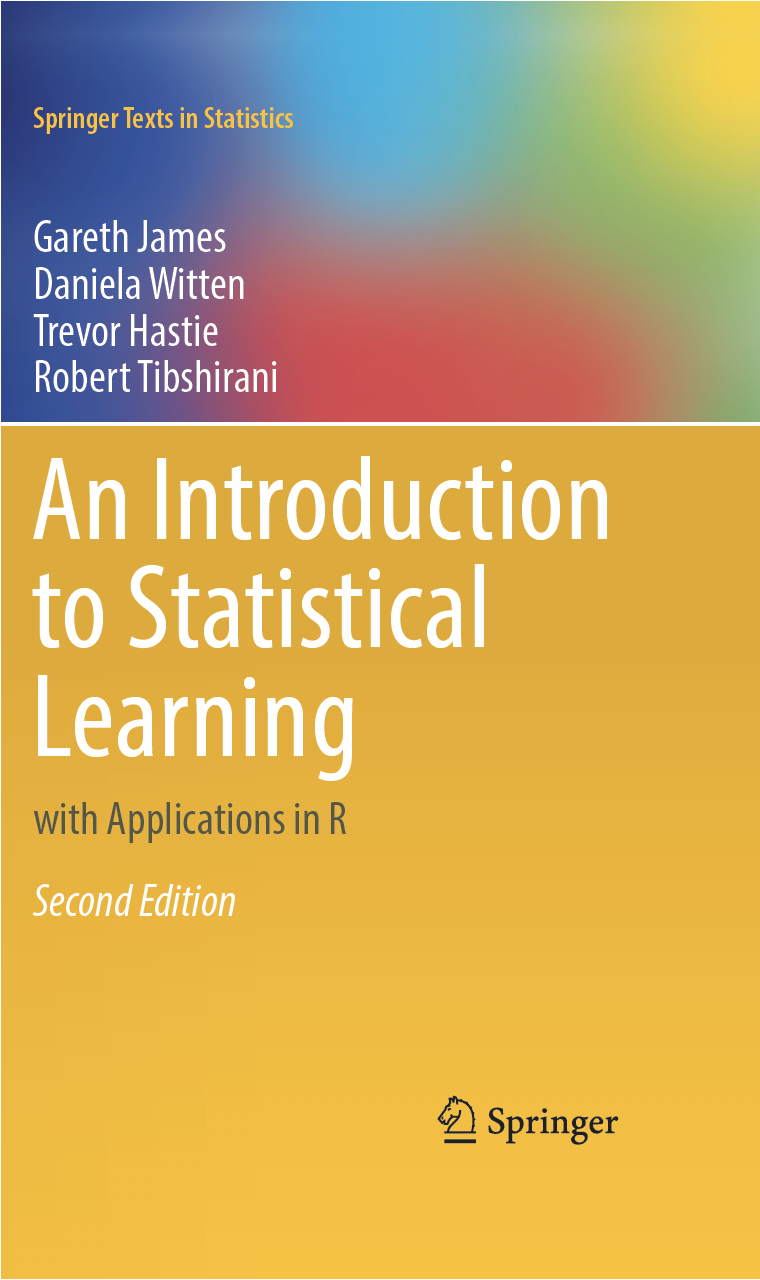
\includegraphics[height = 2in]{images/isl_r.png}
      \end{column}
      \begin{column}{0.5\textwidth}
        \centering
        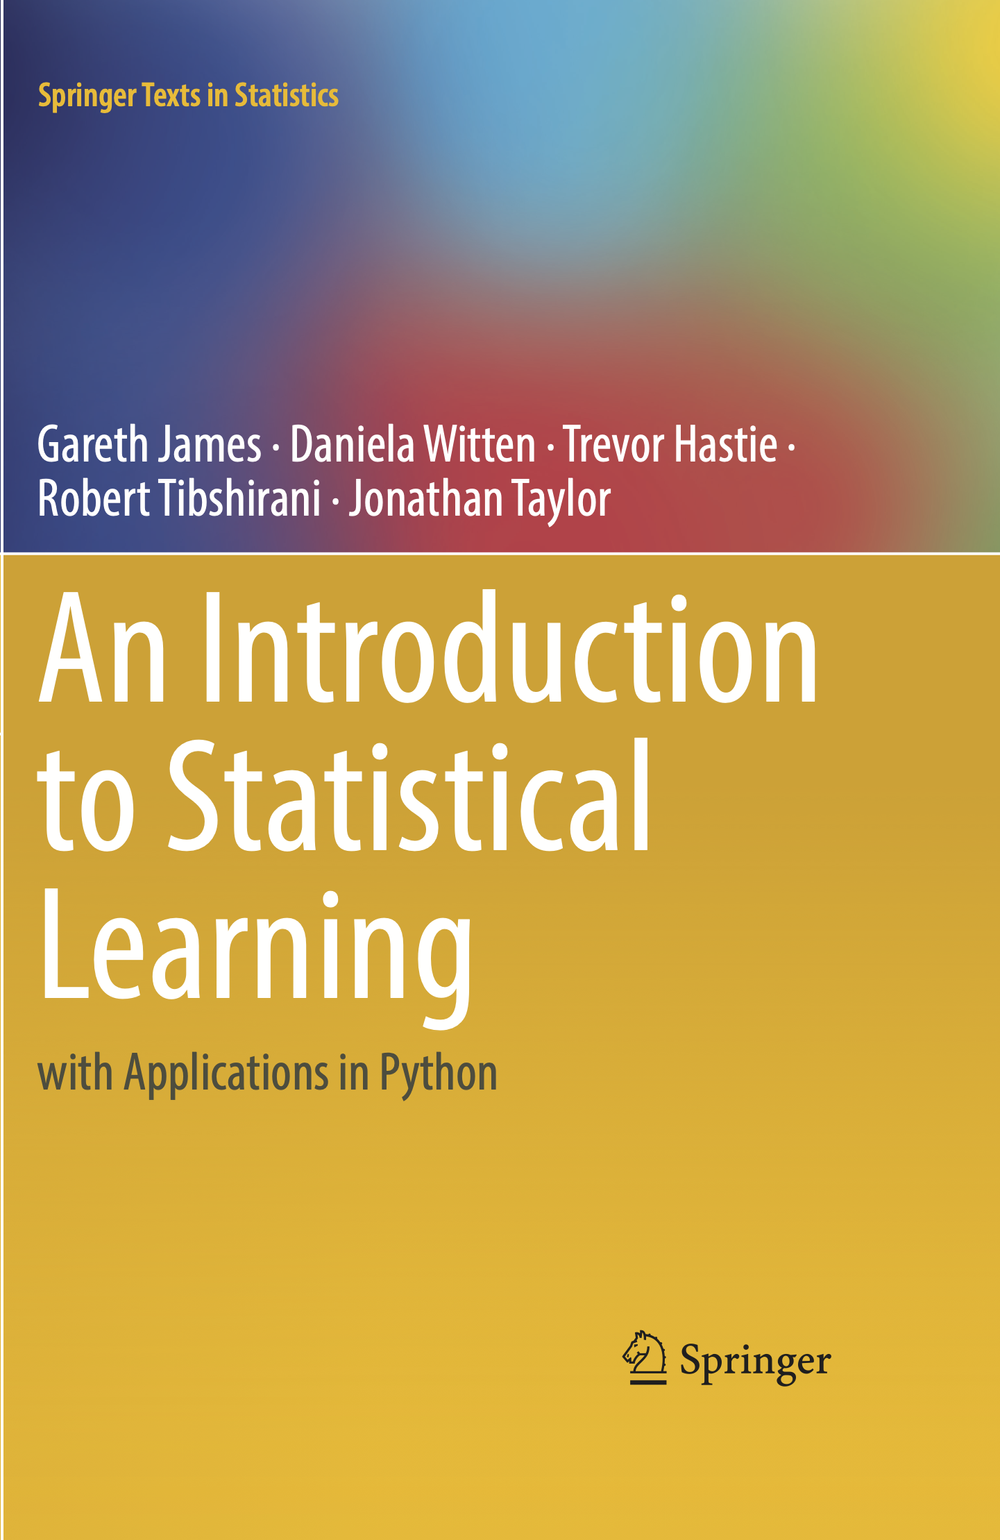
\includegraphics[height = 2in]{images/isl_python.png}
      \end{column}
    \end{columns}
    \vspace{6mm}
    \begin{itemize}
      \item Available for FREE online: \url{statlearning.com}
      \item Today we'll cover mostly Section 6.2 (in R)
    \end{itemize}
  \end{frame}

  \begin{frame}{Linear regression}
    Standard linear model:
    $$Y = \beta_0 + \beta_1 X_1 + ... + \beta_p X_p + \epsilon$$
    Least squares (the typical fitting procedure):
    $$\hat\beta = \arg\min_\beta \left\{ \sum_{i = 1}^n \left(y_i - \beta_0 - \sum_{j = 1}^p \beta_j x_{ij}\right)^2 \right\}$$
    \begin{itemize}
      \item Today we will discuss alternative fitting procedures
      \item Considerations:
      \begin{itemize}
        \item Prediction accuracy
        \item Model interpretability
      \end{itemize}
    \end{itemize}
  \end{frame}

  \begin{frame}{Preview: The Credit data set}
    \centering
    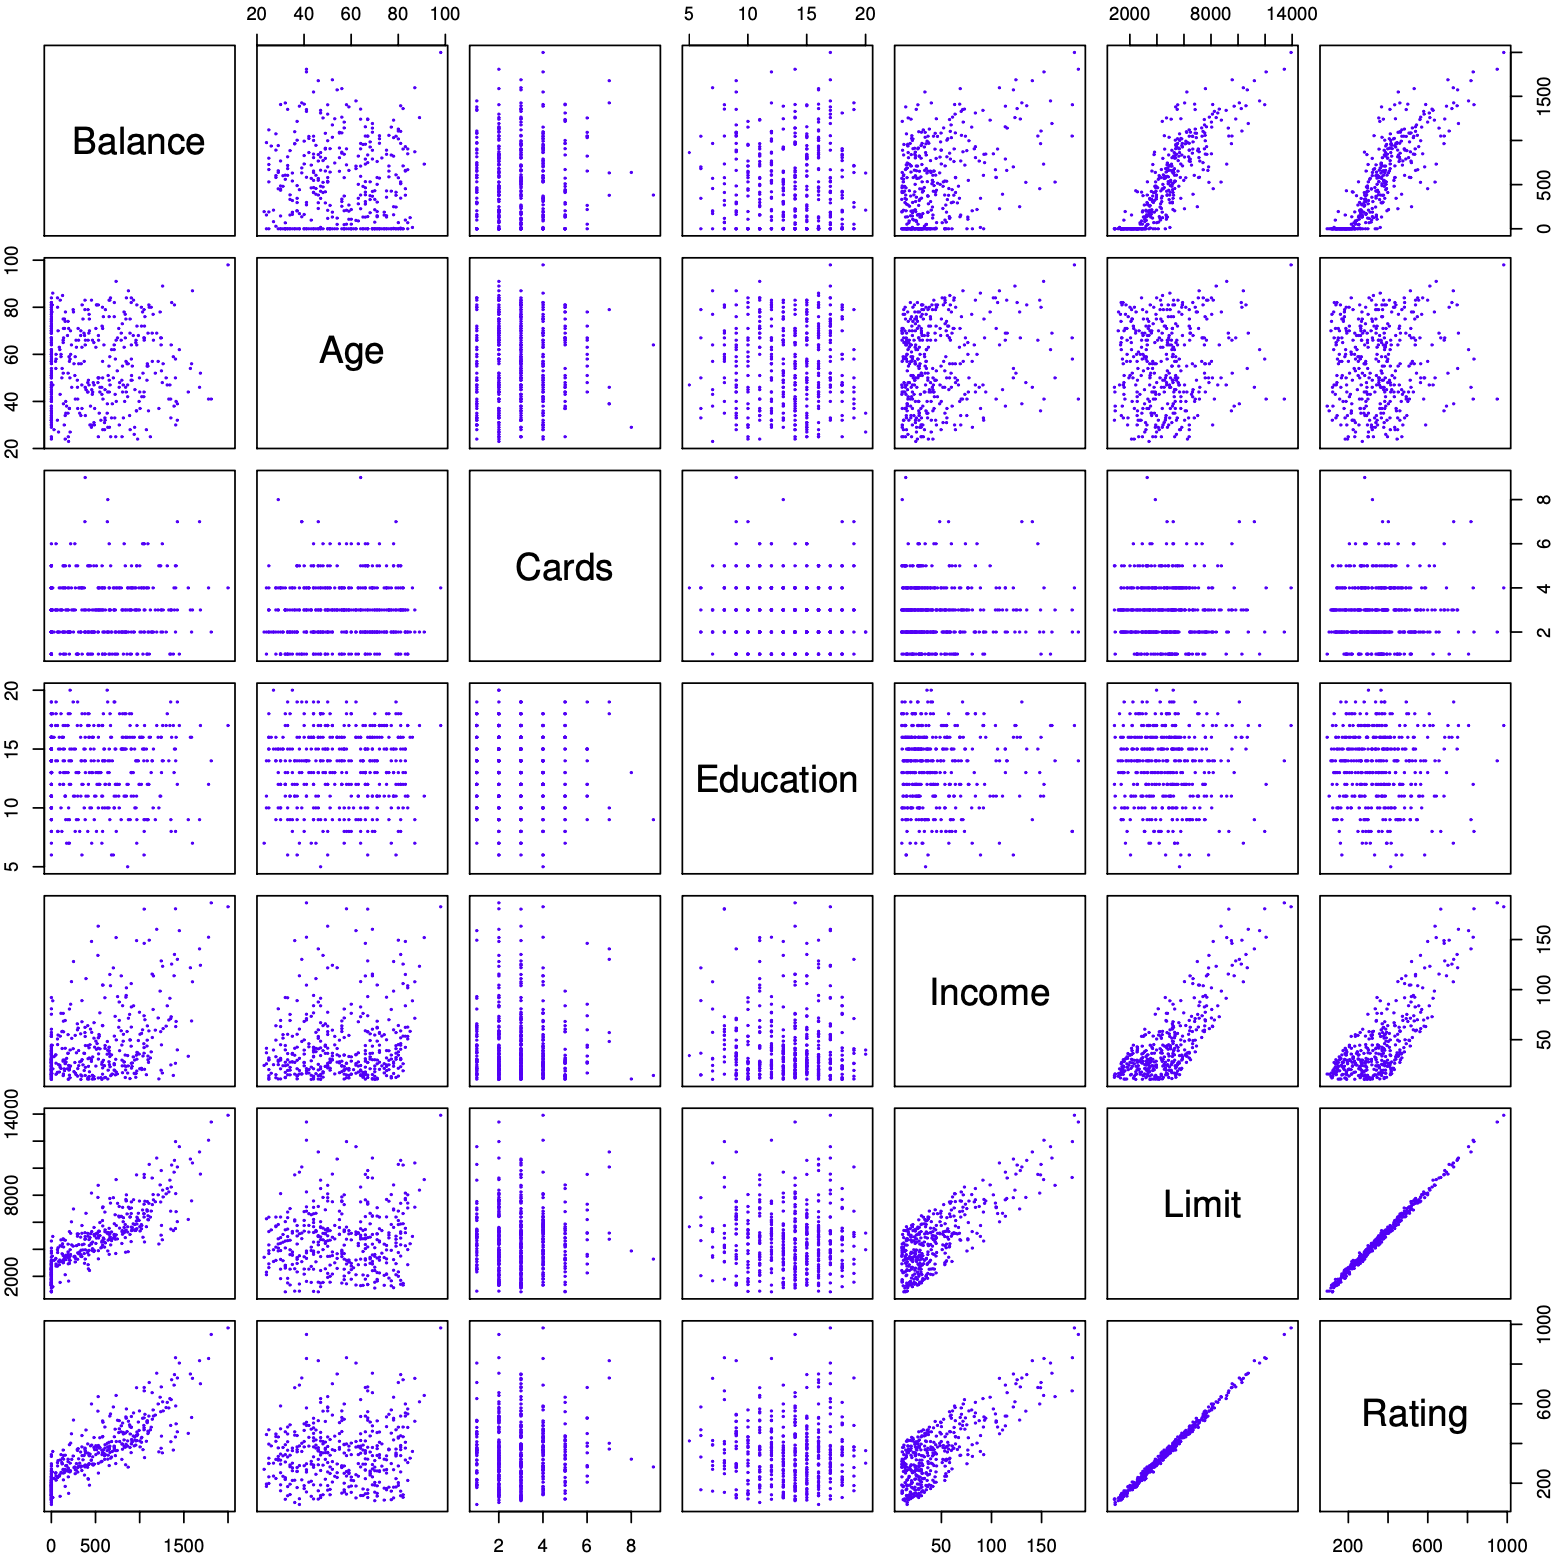
\includegraphics[height = 0.84\textheight]{images/credit.png}
    \footnotesize Credit: ISLR, page 84
  \end{frame}

  \begin{frame}{Alternative \#1: Best subset selection}
    Idea: Select the best model from among the $2^p$ possible models (according to which variables are included in the model)\\
    ~\\
    Algorithm:
    \begin{enumerate}
      \item Let $\mathcal{M}_0$ denote the {\it null model}, which contains no predictors. This model predicts the sample mean for each observation.
      \item For $k = 1, 2, ..., p$:
      \begin{itemize}
        \item[(a)] Fit all $\binom{p}{k}$ models that contain exactly $k$ predictors.
        \item[(b)] Pick the best among these $\binom{p}{k}$ models, and call it $\mathcal{M}_k$.\\
          Best is defined as having the highest $R^2$.
      \end{itemize}
      \item Select a single best model from among $\mathcal{M}_0, ..., \mathcal{M}_p$ using using adjusted $R^2$ or some alternative criterion (e.g. $C_p$, BIC).
    \end{enumerate}
    \begin{itemize}
      \item Computationally infeasible for $p > 40$ (trillions of models)
    \end{itemize}
  \end{frame}

  \begin{frame}{Example: Best subset selection on Credit data set}
    \centering
    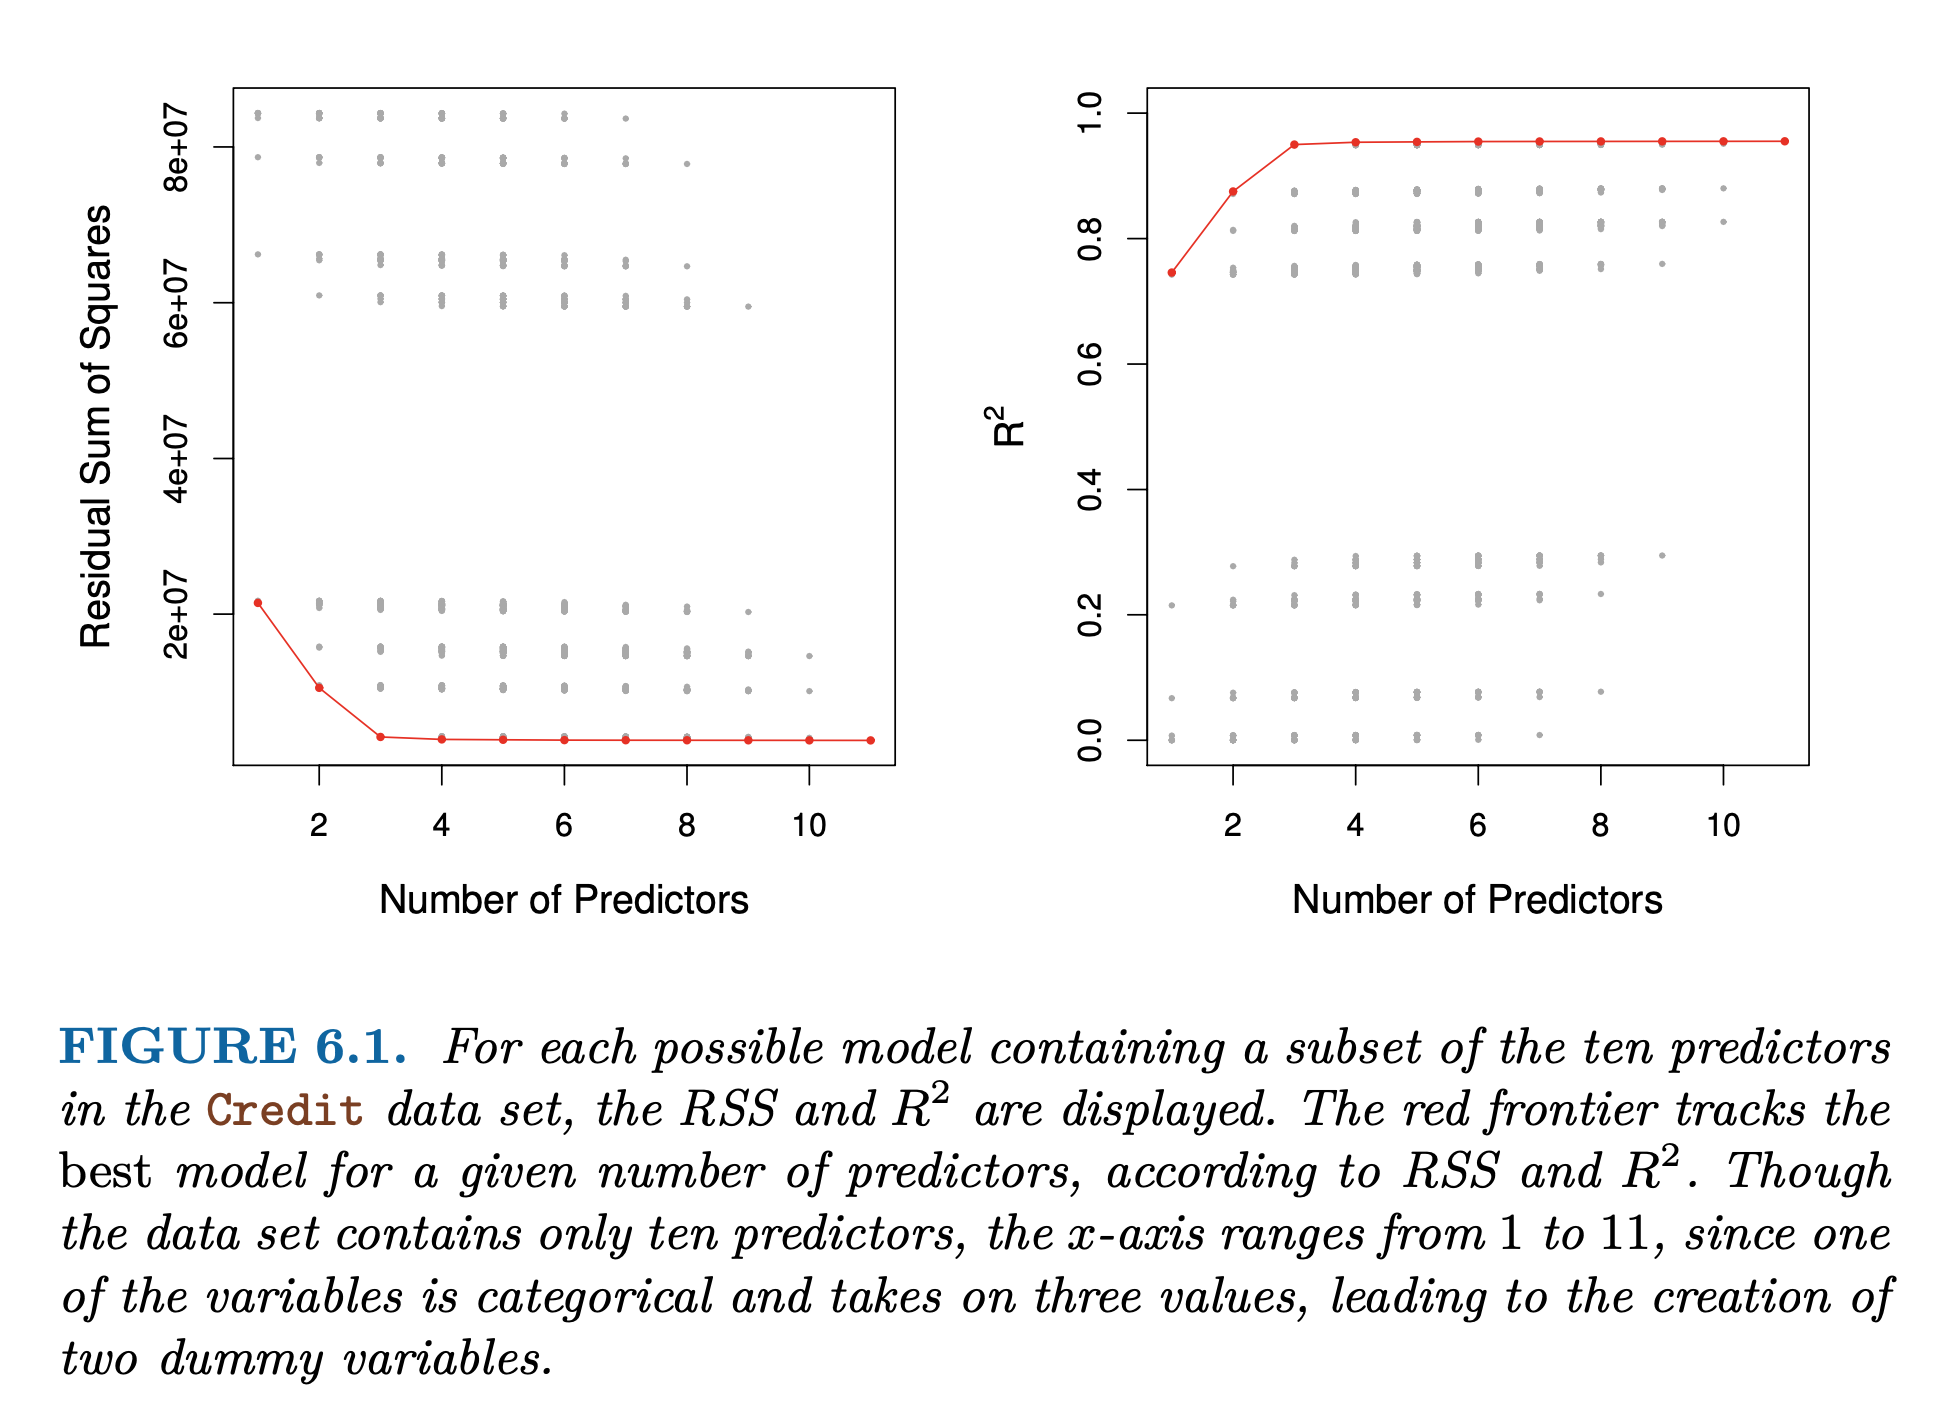
\includegraphics[width = 0.9\textwidth]{images/best_subset_selection.png}
    \vfill
    \hfill \footnotesize Credit: ISLR, page 229
  \end{frame}

  \begin{frame}{Example: Best subset selection on Credit data set}
    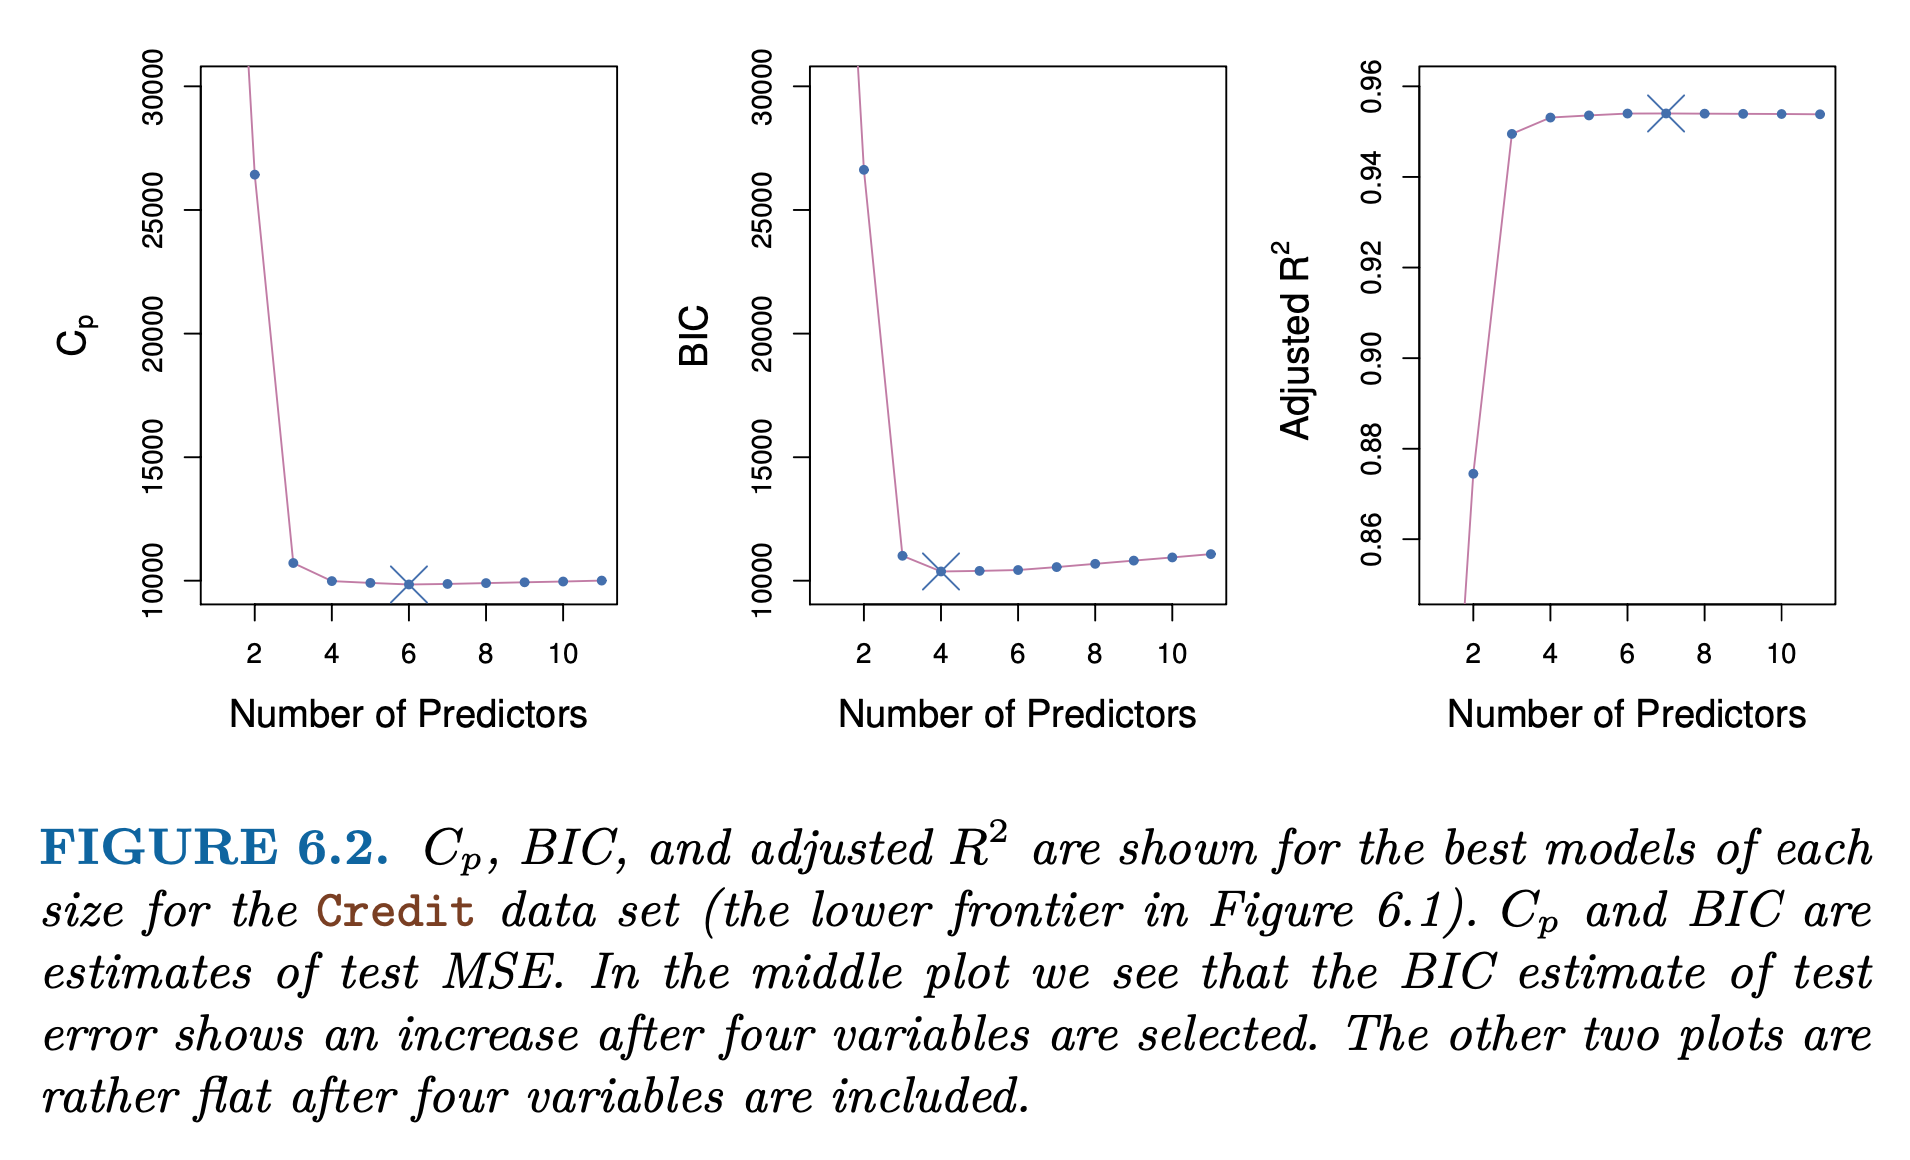
\includegraphics[width = \textwidth]{images/subset_selection_validation.png}
    \vfill
    \hfill \footnotesize Credit: ISLR, page 233
  \end{frame}

  \begin{frame}{Alternative \#2: Backward stepwise selection}
    Idea: Approximate best subset selection with something feasible\\
    ~\\
    Algorithm:
    \begin{enumerate}
      \item Let $\mathcal{M}_p$ denote the full model, which contains all $p$ predictors.
      \item For $k = p, p-1, ..., 1$:
      \begin{itemize}
        \item[(a)] Consider all $k$ models that contain all but one of the predictors in $\mathcal{M}_k$, for a total of $k-1$ predictors.
        \item[(b)] Choose the best among these $k$ models, and call it $\mathcal{M}_{k-1}$. Best is defined as having the highest $R^2$.
      \end{itemize}
      \item Select a single best model from among $\mathcal{M}_0, ..., \mathcal{M}_p$ using using adjusted $R^2$ or some alternative criterion (e.g. $C_p$, BIC).
    \end{enumerate}
    \begin{itemize}
      \item Similar to repeatedly dropping predictor with highest $p$-value
    \end{itemize}
  \end{frame}

  \begin{frame}{Alternative \#3: Ridge regression}
    Least squares:
    $$\hat\beta = \arg\min_\beta \left\{ \sum_{i = 1}^n \left(y_i - \beta_0 - \sum_{j = 1}^p \beta_j x_{ij}\right)^2 \right\}$$
    Ridge regression:
    $$\hat\beta^R_\lambda = \arg\min_\beta \left\{ \sum_{i = 1}^n \left(y_i - \beta_0 - \sum_{j = 1}^p \beta_j x_{ij}\right)^2 + \lambda \sum_{j = 1}^p \beta_j^2 \right\}$$
    \hfill $\lambda \ge 0$ is a {\it tuning parameter}
    \begin{itemize}
      \item Ridge regression introduces a {\it shrinkage penalty}
      \item Computation is very fast (similar to least squares)
    \end{itemize}
  \end{frame}

  \begin{frame}{Example: Ridge regression on Credit data set}
    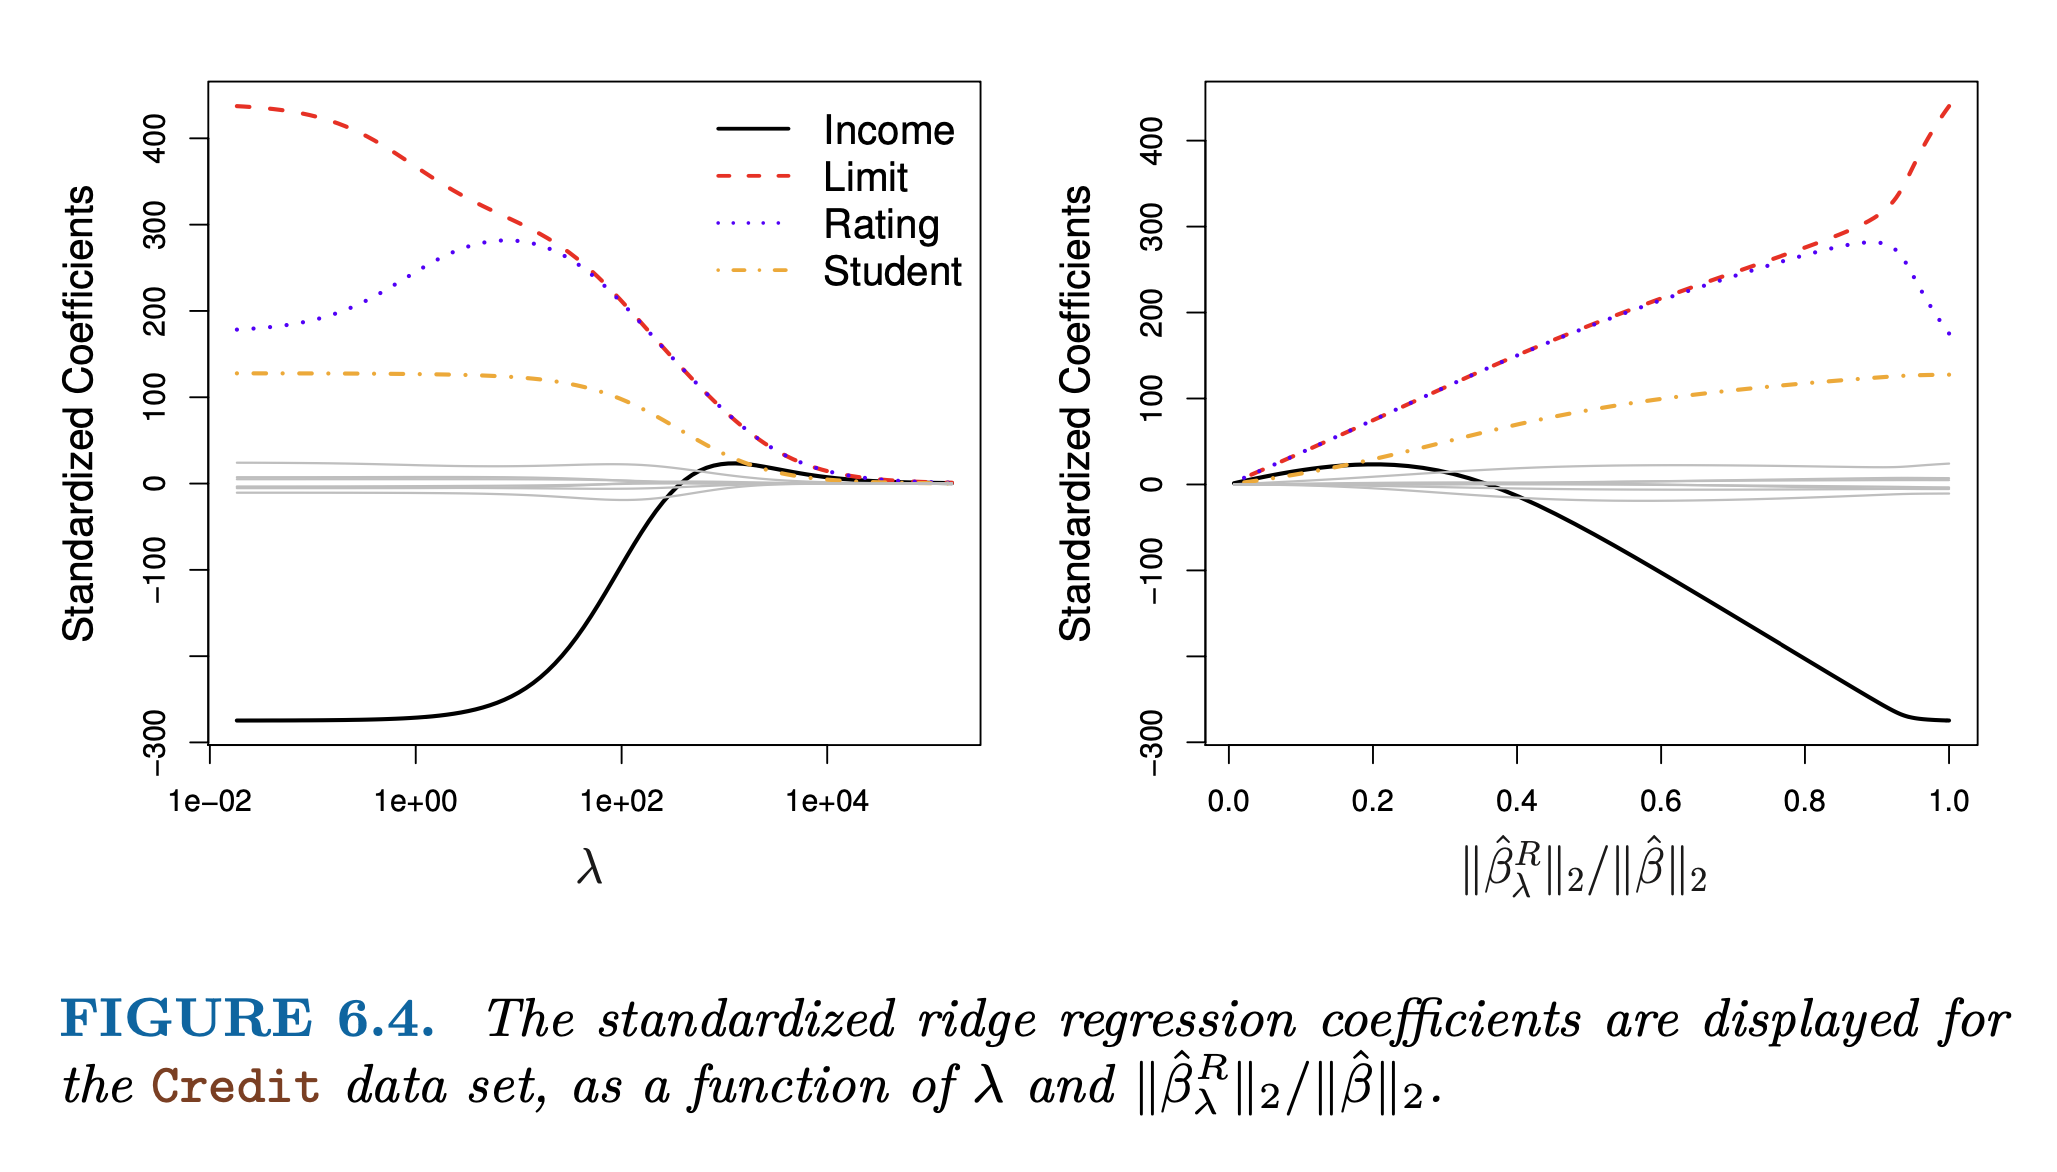
\includegraphics[width = \textwidth]{images/ridge_credit.png}
    \vfill
    \hfill \footnotesize Credit: ISLR, page 238
  \end{frame}

  \begin{frame}{The bias-variance trade-off}
    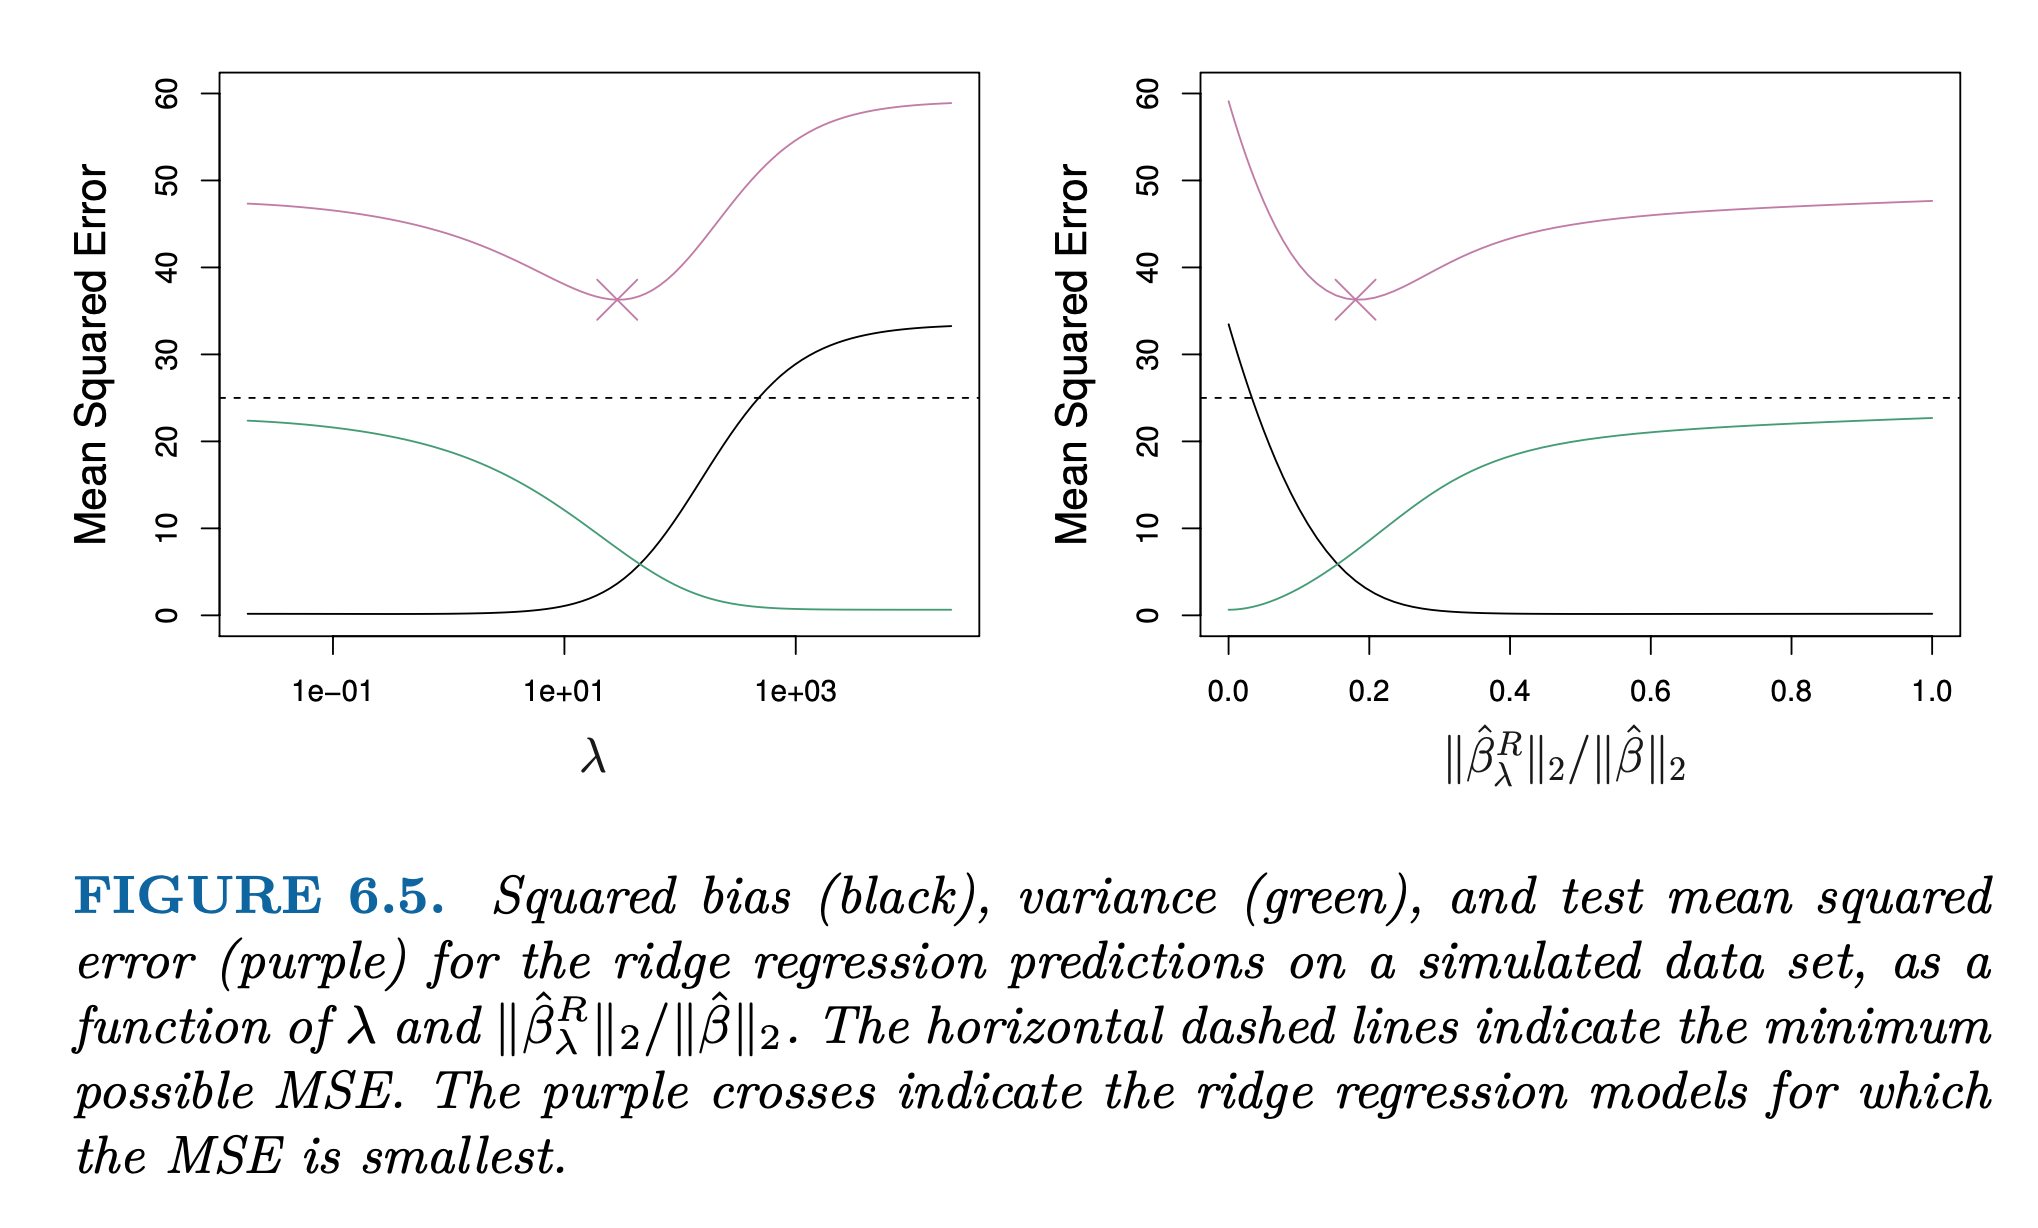
\includegraphics[width = \textwidth]{images/bias_variance.png}
    \vfill
    \hfill \footnotesize Credit: ISLR, page 240
  \end{frame}

  \begin{frame}{Exercise (ISLR, page 284)}
    \footnotesize
    Suppose we estimate the coefficients in a linear regression model by minimizing
    $$\sum_{i = 1}^n \left(y_i - \beta_0 - \sum_{j = 1}^p \beta_j x_{ij}\right)^2 + \lambda \sum_{j = 1}^p \beta_j^2$$
    \begin{itemize}
      \item[(a)] As we increase $\lambda$ from 0, the training RSS will: (choose correct answer)
      \begin{itemize}
        \item[i.] Decrease initially, and then eventually increase in a U shape.
        \item[ii.] Increase initially, and then eventually decrease in an inverted U.
        \item[iii.] Steadily increase.
        \item[iv.] Steadily decrease.
        \item[v.] Remain constant.
      \end{itemize}
      \item[(b)] Repeat (a) for test RSS.
      \item[(c)] Repeat (a) for variance.
      \item[(d)] Repeat (a) for (squared) bias.
    \end{itemize}
  \end{frame}

  \begin{frame}{The lasso}
    $$\hat\beta^L_\lambda = \arg\min_\beta \left\{ \sum_{i = 1}^n \left(y_i - \beta_0 - \sum_{j = 1}^p \beta_j x_{ij}\right)^2 + \lambda \sum_{j = 1}^p |\beta_j| \right\}$$
    \begin{itemize}
      \item Achieves {\it variable selection} (drops some variables from model)
      \item Not as fast as ridge regression, but also very fast
    \end{itemize}
  \end{frame}

  \begin{frame}{Example: The lasso on Credit data set}
    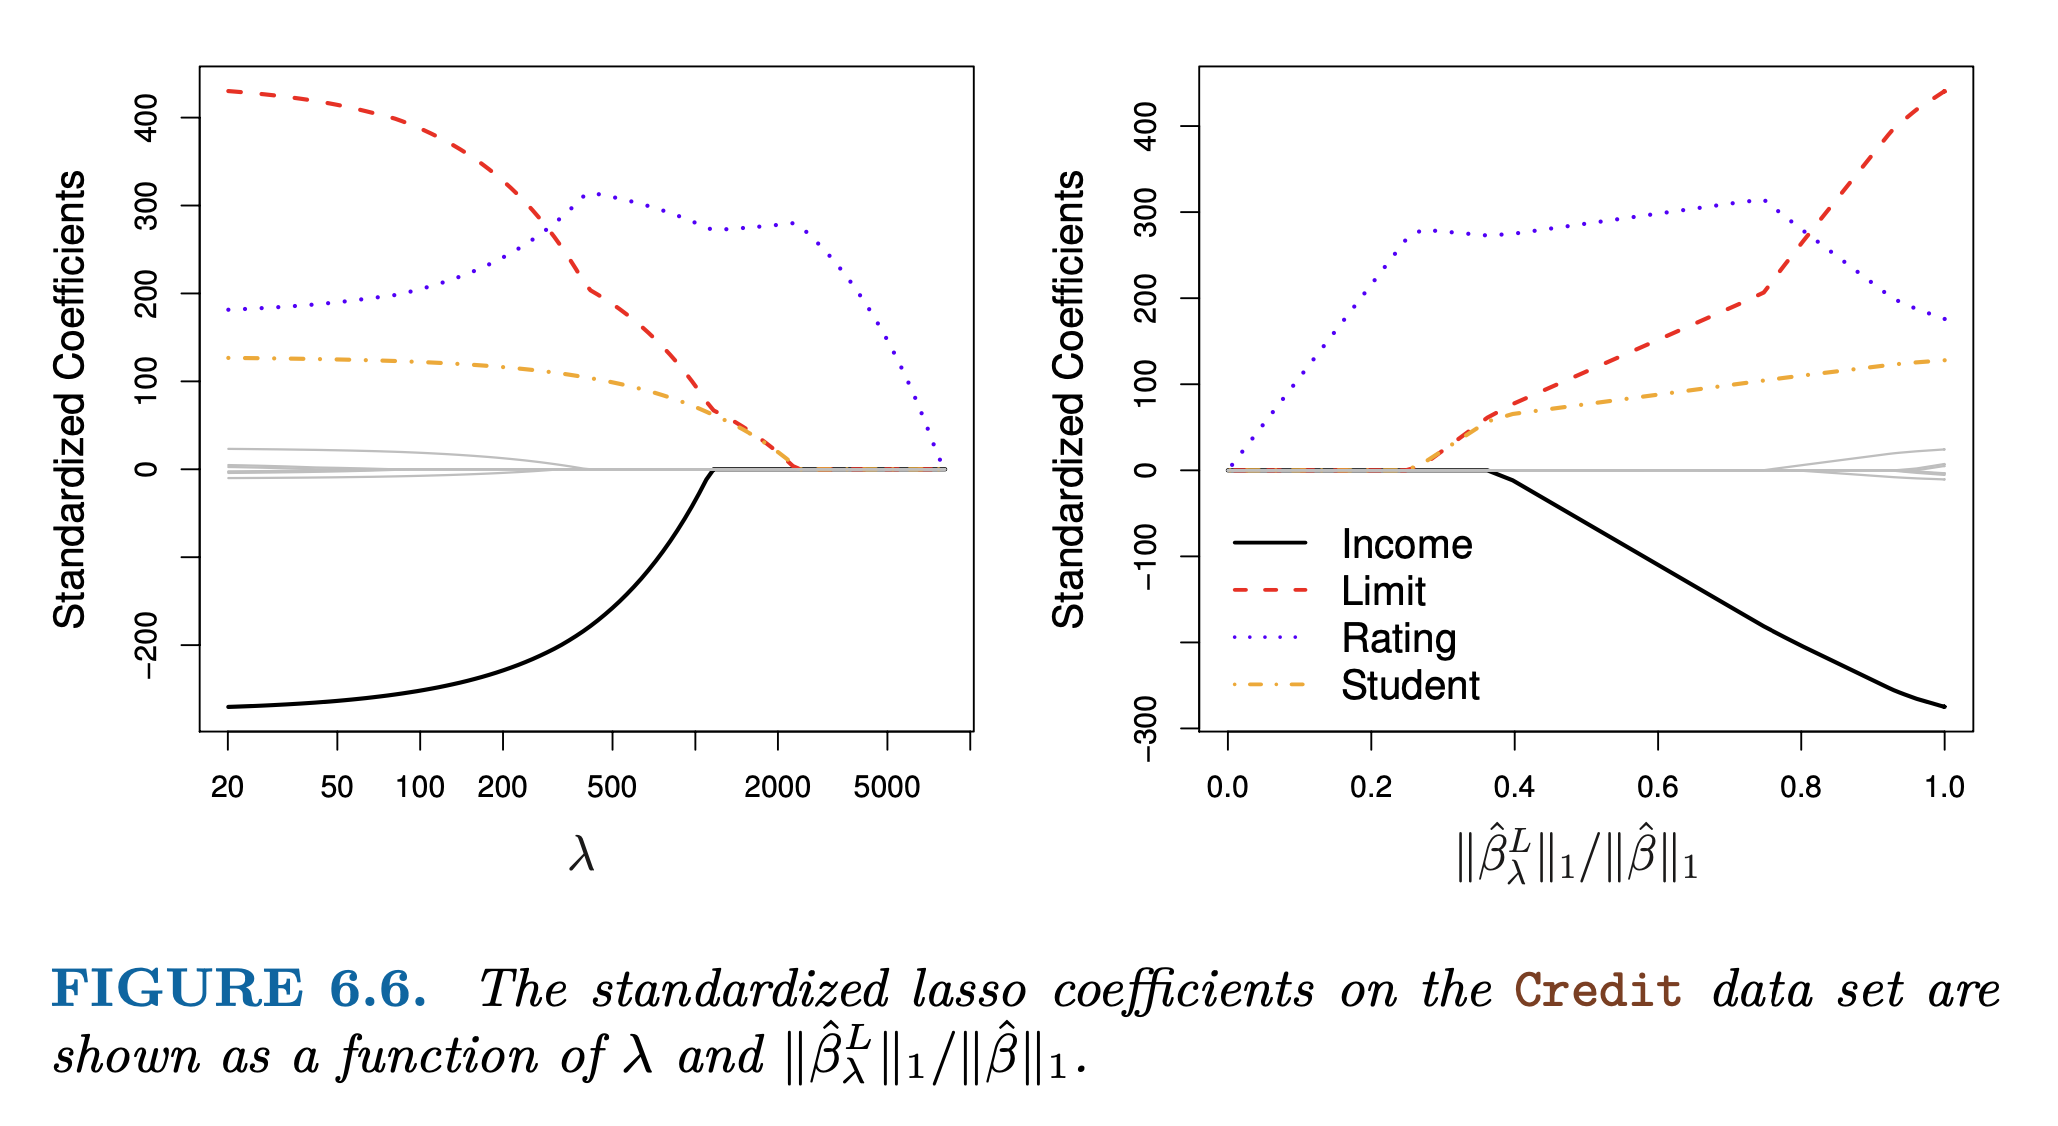
\includegraphics[width = \textwidth]{images/lasso_credit.png}
    \vfill
    \hfill \footnotesize Credit: ISLR, page 243
  \end{frame}

  \begin{frame}{Exercise (ISLR, page 284)}
    The lasso, relative to least squares, is: (choose correct answer)
    \begin{itemize}
      \item[i.] More flexible and hence will give improved prediction accuracy when its increase in bias is less than its decrease in variance.
      \item[ii.] More flexible and hence will give improved prediction accuracy when its increase in variance is less than its decrease in bias.
      \item[iii.] Less flexible and hence will give improved prediction accuracy when its increase in bias is less than its decrease in variance.
      \item[iv.] Less flexible and hence will give improved prediction accuracy when its increase in variance is less than its decrease in bias.
    \end{itemize}
  \end{frame}

  \begin{frame}{Another formulation}
    \small
    Ridge regression:
    $$\hat\beta = \arg\min_\beta \left\{ \sum_{i = 1}^n \left(y_i - \beta_0 - \sum\beta_j x_{ij}\right)^2 \right\} \mbox{ s.t. } \sum_{j = 1}^p \beta_j^2 \le s$$
    The lasso:
    $$\hat\beta = \arg\min_\beta \left\{ \sum_{i = 1}^n \left(y_i - \beta_0 - \sum\beta_j x_{ij}\right)^2 \right\} \mbox{ s.t. } \sum_{j = 1}^p |\beta_j| \le s$$
    Best subset selection:
    $$\hat\beta = \arg\min_\beta \left\{ \sum_{i = 1}^n \left(y_i - \beta_0 - \sum\beta_j x_{ij}\right)^2 \right\} \mbox{ s.t. } \sum_{j = 1}^p \mathbb{I}(\beta_j \ne 0) \le s$$
  \end{frame}

  \begin{frame}{Variable selection by the lasso}
    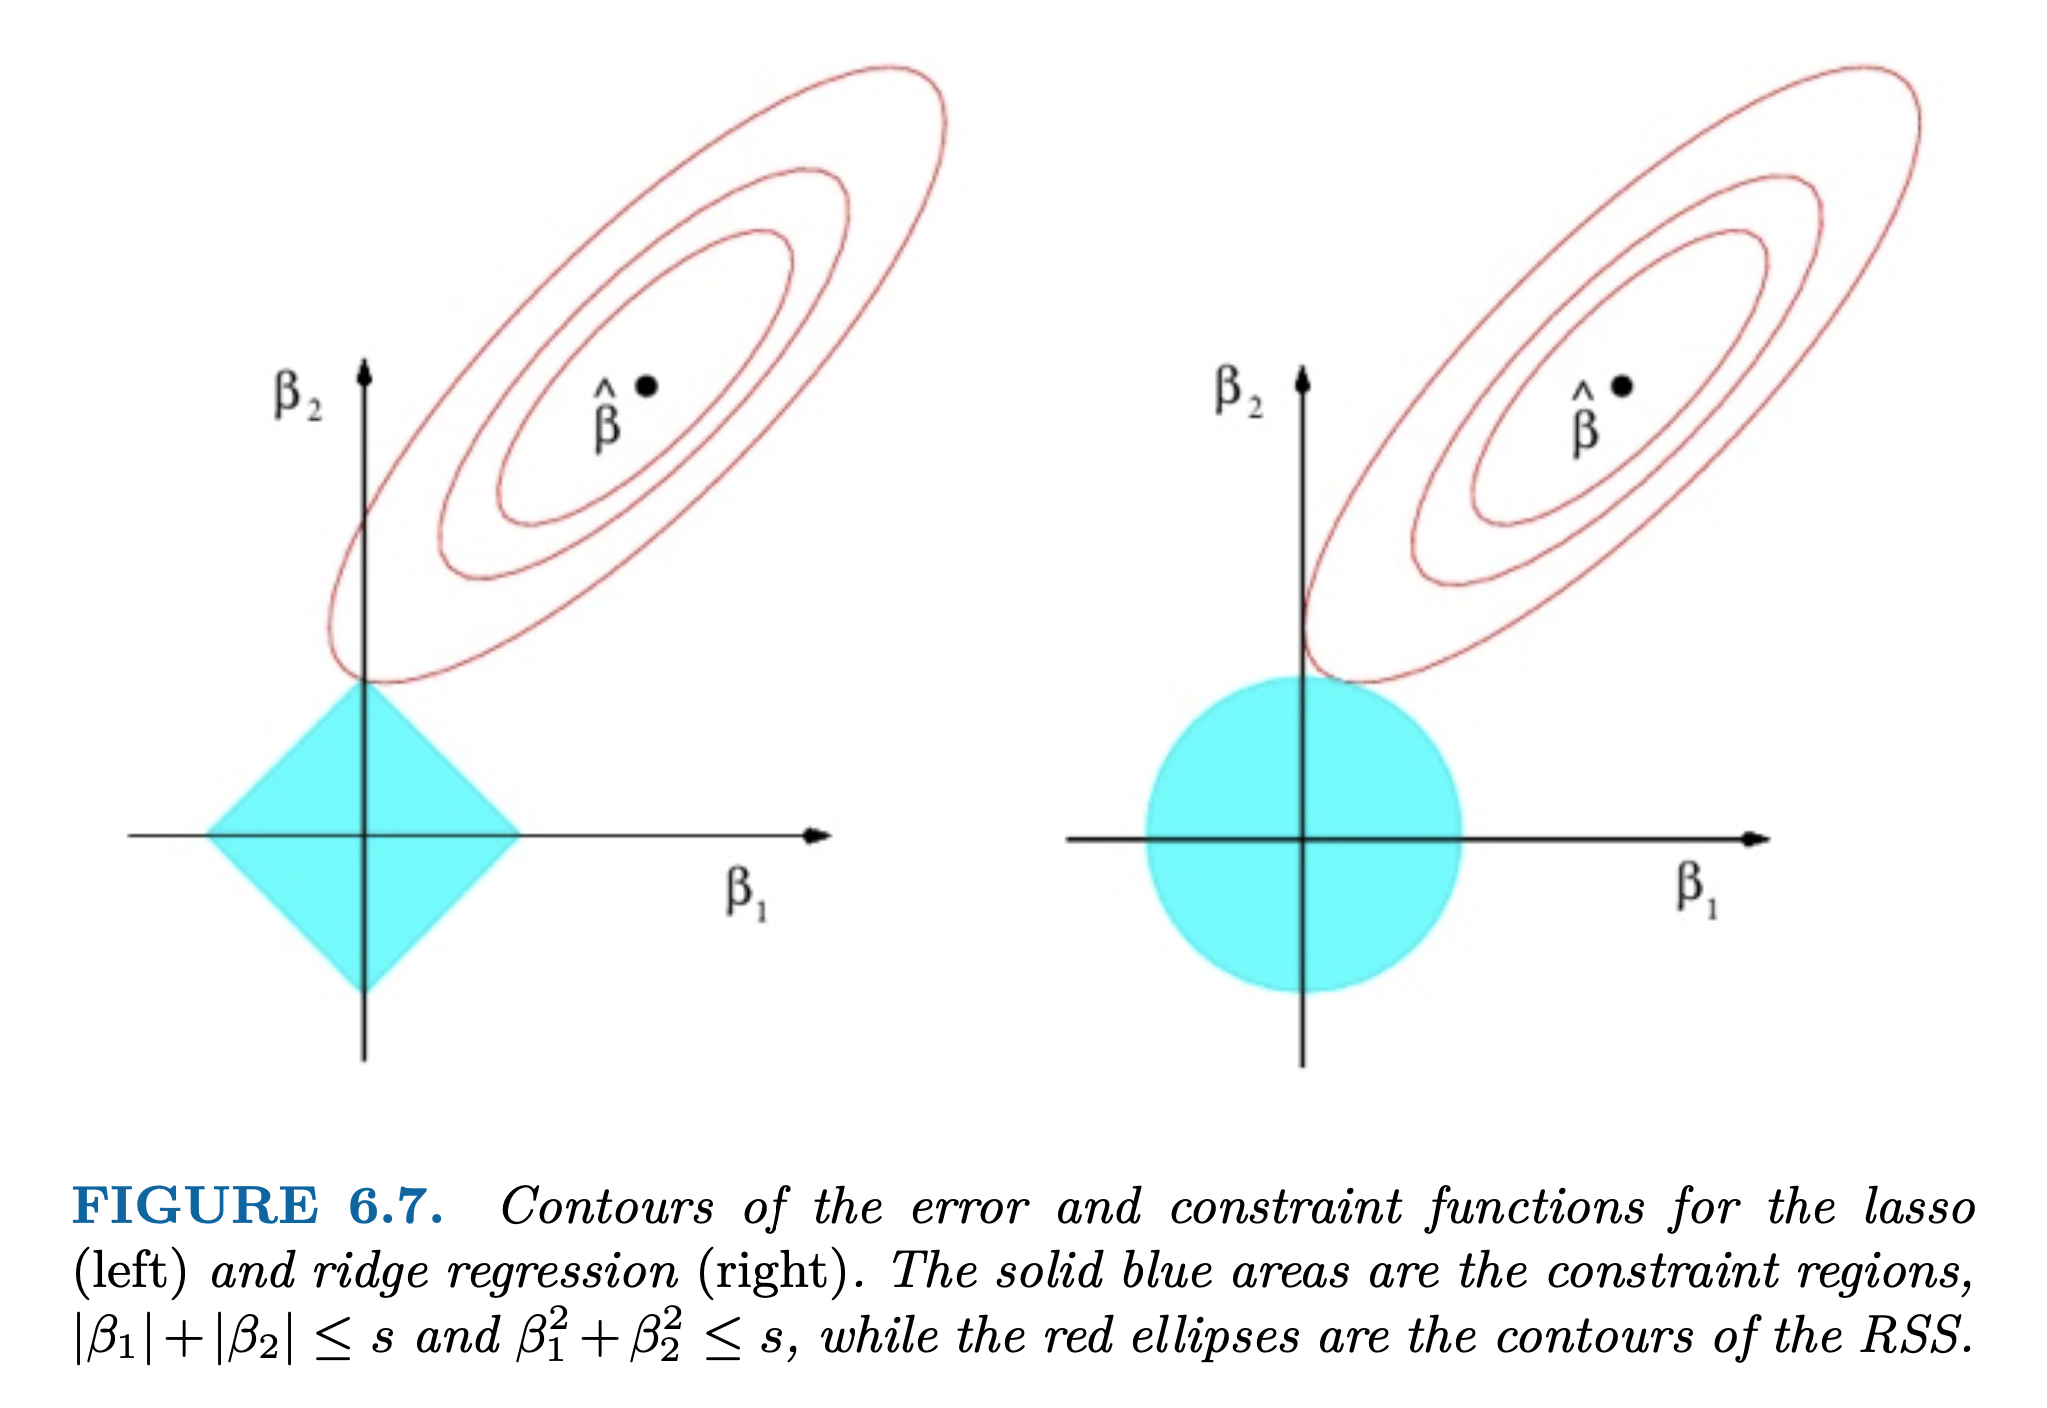
\includegraphics[width = \textwidth]{images/variable_selection.png}
    \vfill
    \hfill \footnotesize Credit: ISLR, page 245
  \end{frame}

  \begin{frame}{A simple special case}
    \begin{center}
      $n = p$, one coefficent $\beta_j$ corresponding to each observation $y_j$\\
    \end{center}
    Least squares:
    $$\sum_{j = 1}^p(y_j - \beta_j)^2 \quad \Rightarrow \quad \hat \beta_j = y_j$$
    Ridge regression:
    $$\sum_{j = 1}^p(y_j - \beta_j)^2 + \lambda \sum_{j = 1}^p \beta_j^2 \quad \Rightarrow \quad \hat \beta_j^R = y_j / (1 + \lambda)$$\\
    The lasso:
    $$\sum_{j = 1}^p(y_j - \beta_j)^2 + \lambda \sum_{j = 1}^p |\beta_j| \quad \Rightarrow \quad \hat \beta_j^L = \begin{cases}
      y_j - \lambda/2 & \mbox{if }y_j > \lambda / 2\\
      y_j + \lambda/2 & \mbox{if }y_j < -\lambda / 2\\
      0               & \mbox{if }|y_j| \le \lambda / 2\\
    \end{cases}$$\\
  \end{frame}

  \begin{frame}{A simple special case}
    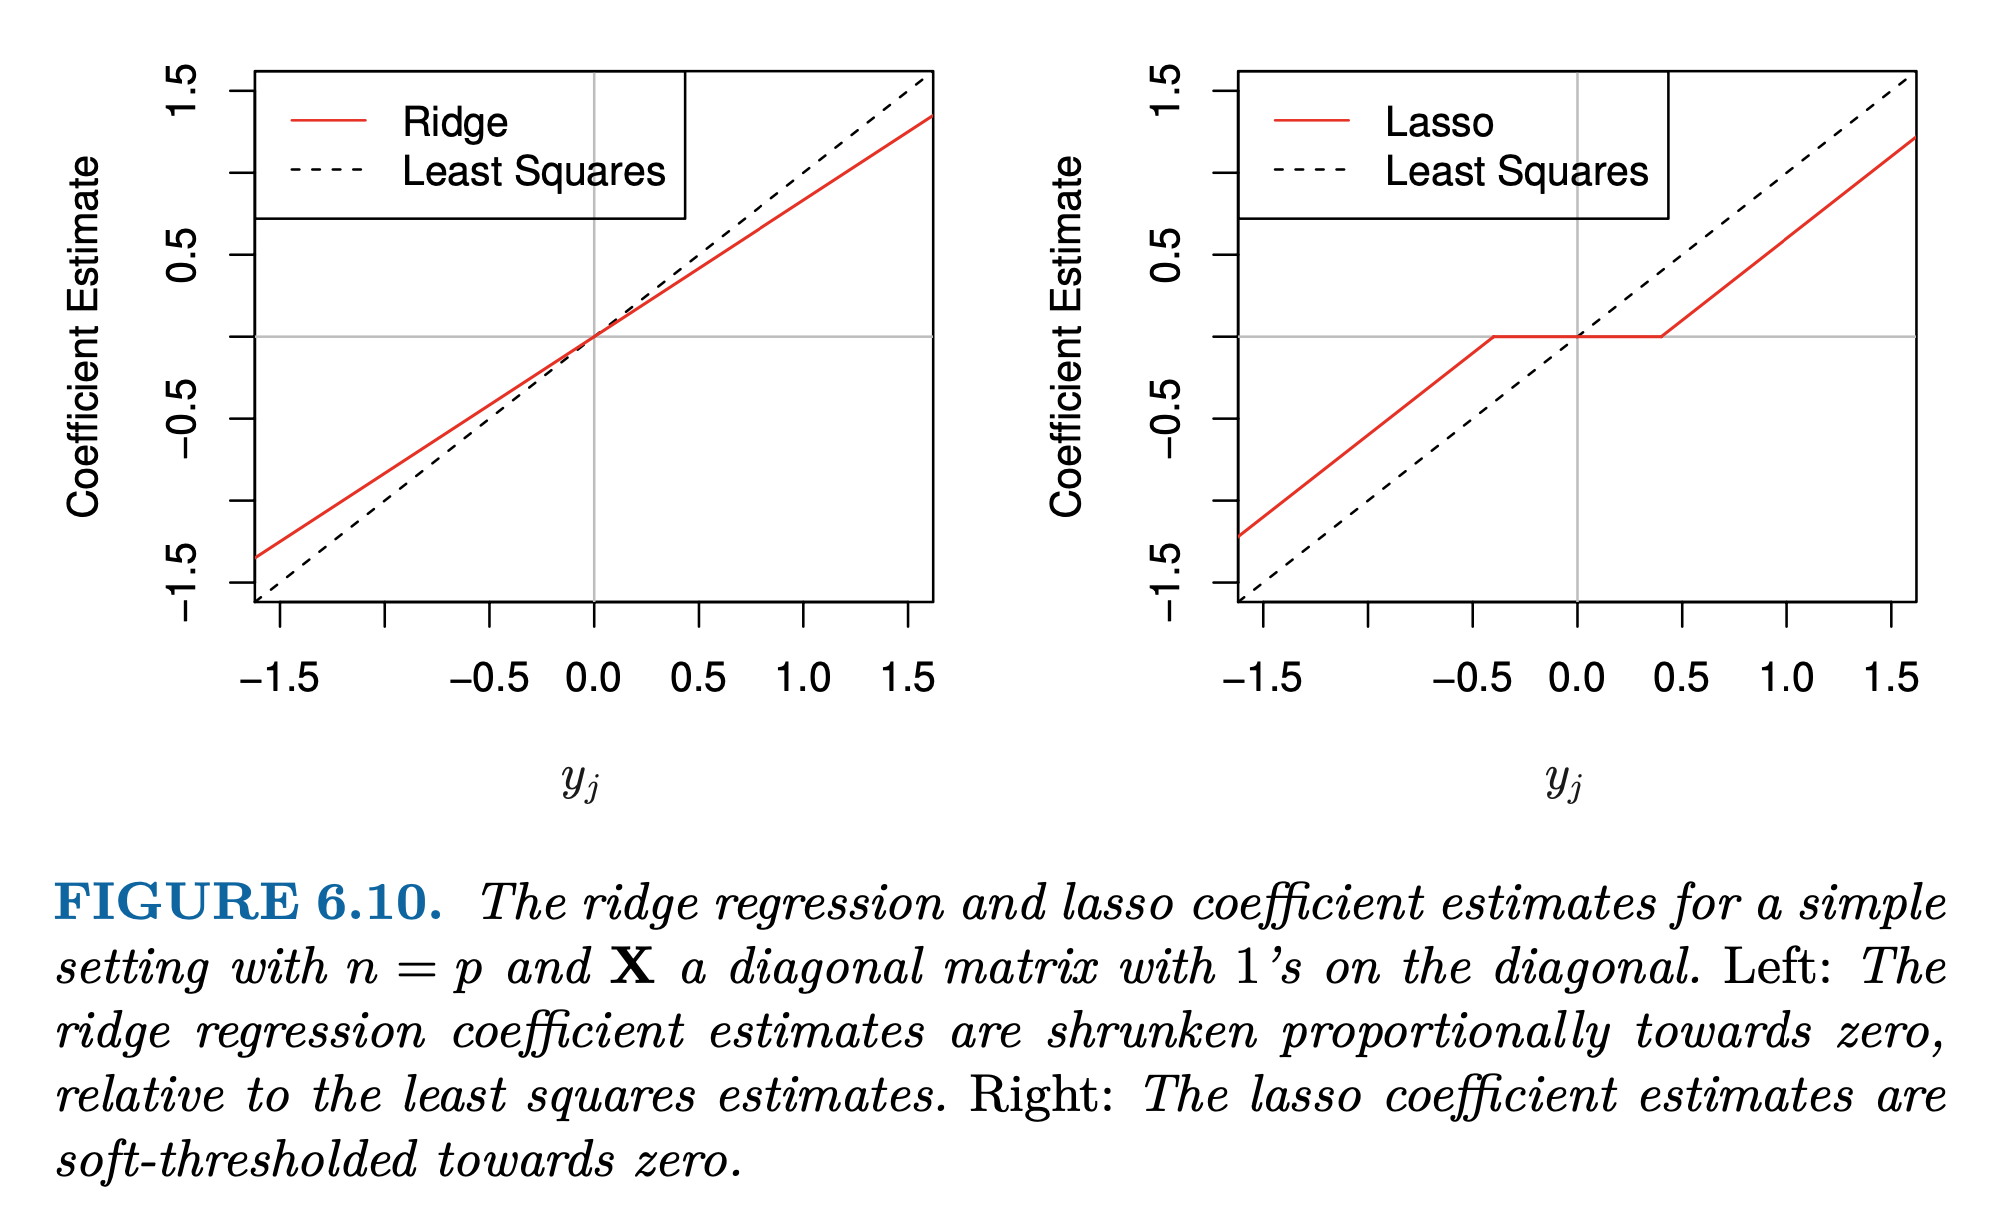
\includegraphics[width = \textwidth]{images/simple_special_case.png}
    \vfill
    \hfill \footnotesize Credit: ISLR, page 248
  \end{frame}

  \begin{frame}{Exercise (ISLR, page 285)}
    \small
    \begin{itemize}
      \item[(a)] Assume $p = 1$. For some choice of $y_1$ and $\lambda > 0$, plot
        \begin{equation}
          \label{eqn:ridge-simple}
          \sum_{j = 1}^p(y_j - \beta_j)^2 + \lambda \sum_{j = 1}^p \beta_j^2
        \end{equation}
        as a function of $\beta_1$. Your plot should agree that (\ref{eqn:ridge-simple}) is minimized by
        $$\hat \beta_j^R = y_j / (1 + \lambda).$$
      \item[(b)] Assume $p = 1$. For some choice of $y_1$ and $\lambda > 0$, plot
        \begin{equation}
          \label{eqn:lasso-simple}
          \sum_{j = 1}^p(y_j - \beta_j)^2 + \lambda \sum_{j = 1}^p |\beta_j|
        \end{equation}
        as a function of $\beta_1$. Your plot should agree that (\ref{eqn:lasso-simple}) is minimized by

        $$
          \hat \beta_j^L = \begin{cases}
            y_j - \lambda/2 & \mbox{if }y_j > \lambda / 2\\
            y_j + \lambda/2 & \mbox{if }y_j < -\lambda / 2\\
            0               & \mbox{if }|y_j| \le \lambda / 2
          \end{cases}.
        $$
    \end{itemize}
  \end{frame}

  \begin{frame}{Selecting the tuning parameter}
    How to select the tuning parameter $\lambda$?\\
    ~\\
    Validation set approach:\\
    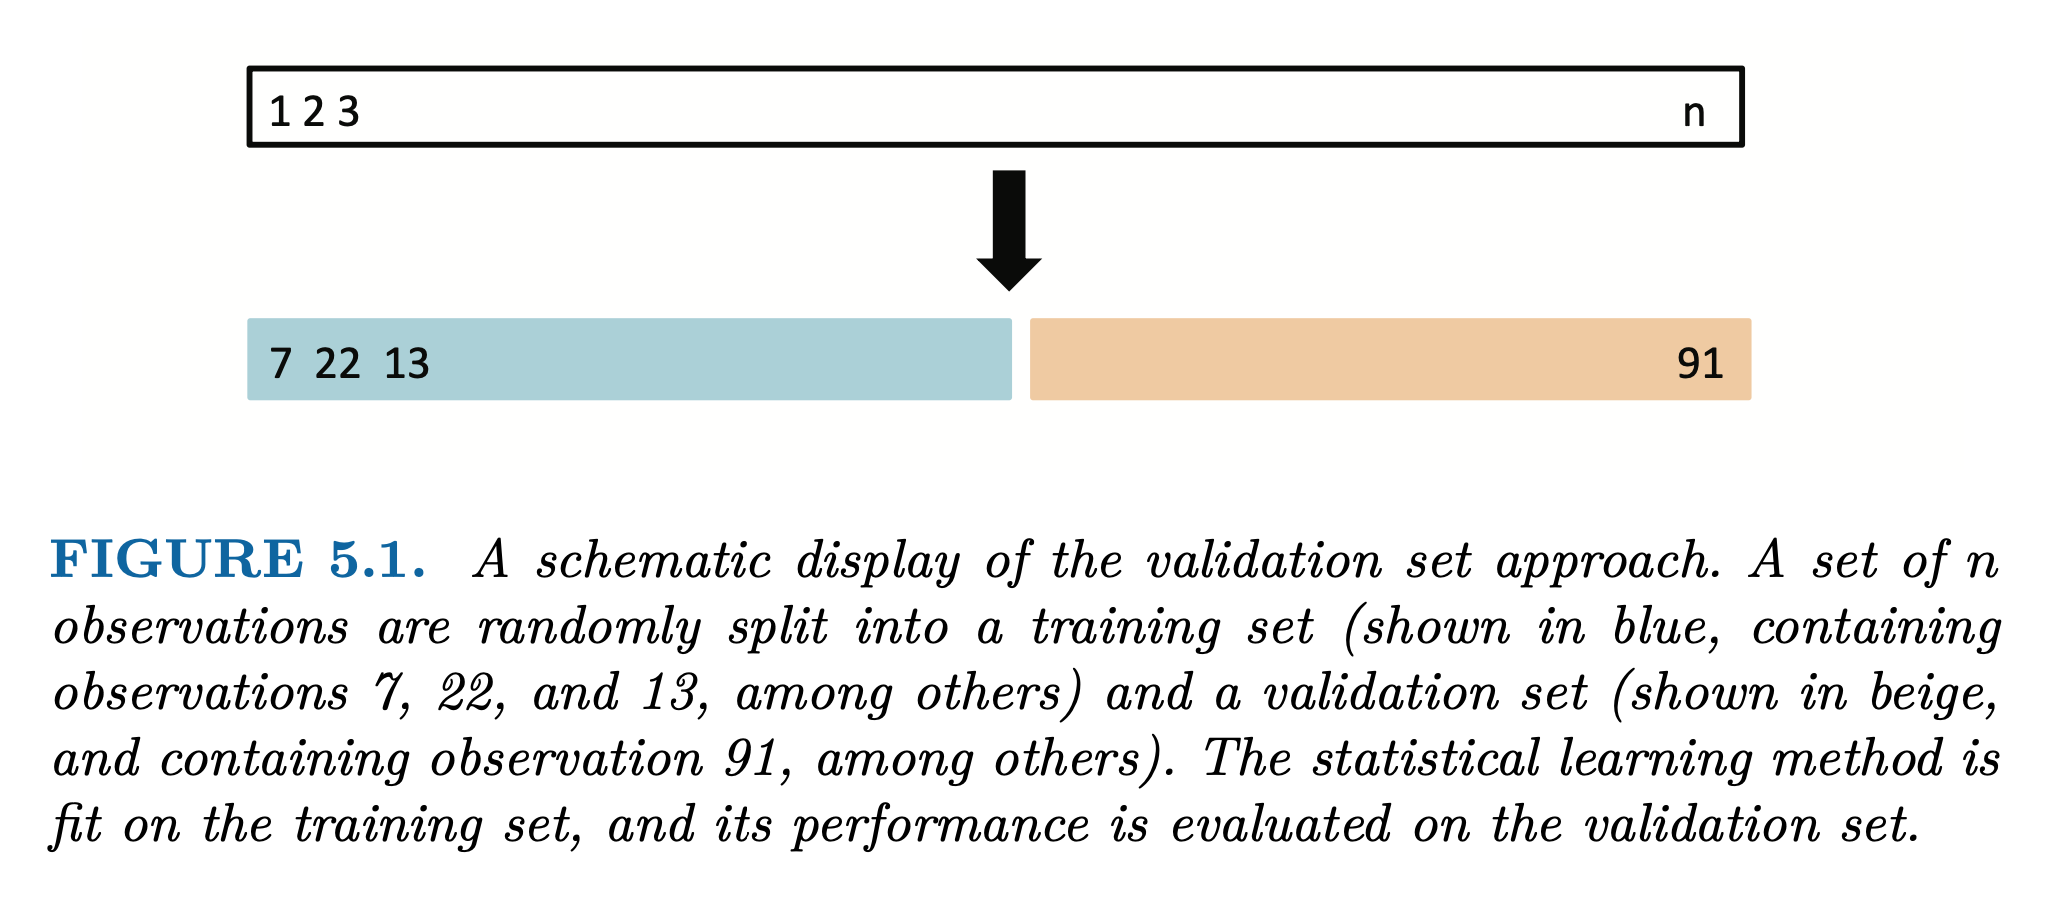
\includegraphics[width = \textwidth]{images/validation_set.png}\\
    \hfill \footnotesize Credit: ISLR, page 199
  \end{frame}

  \begin{frame}{Leave-one-out cross-validation (LOOCV)}
    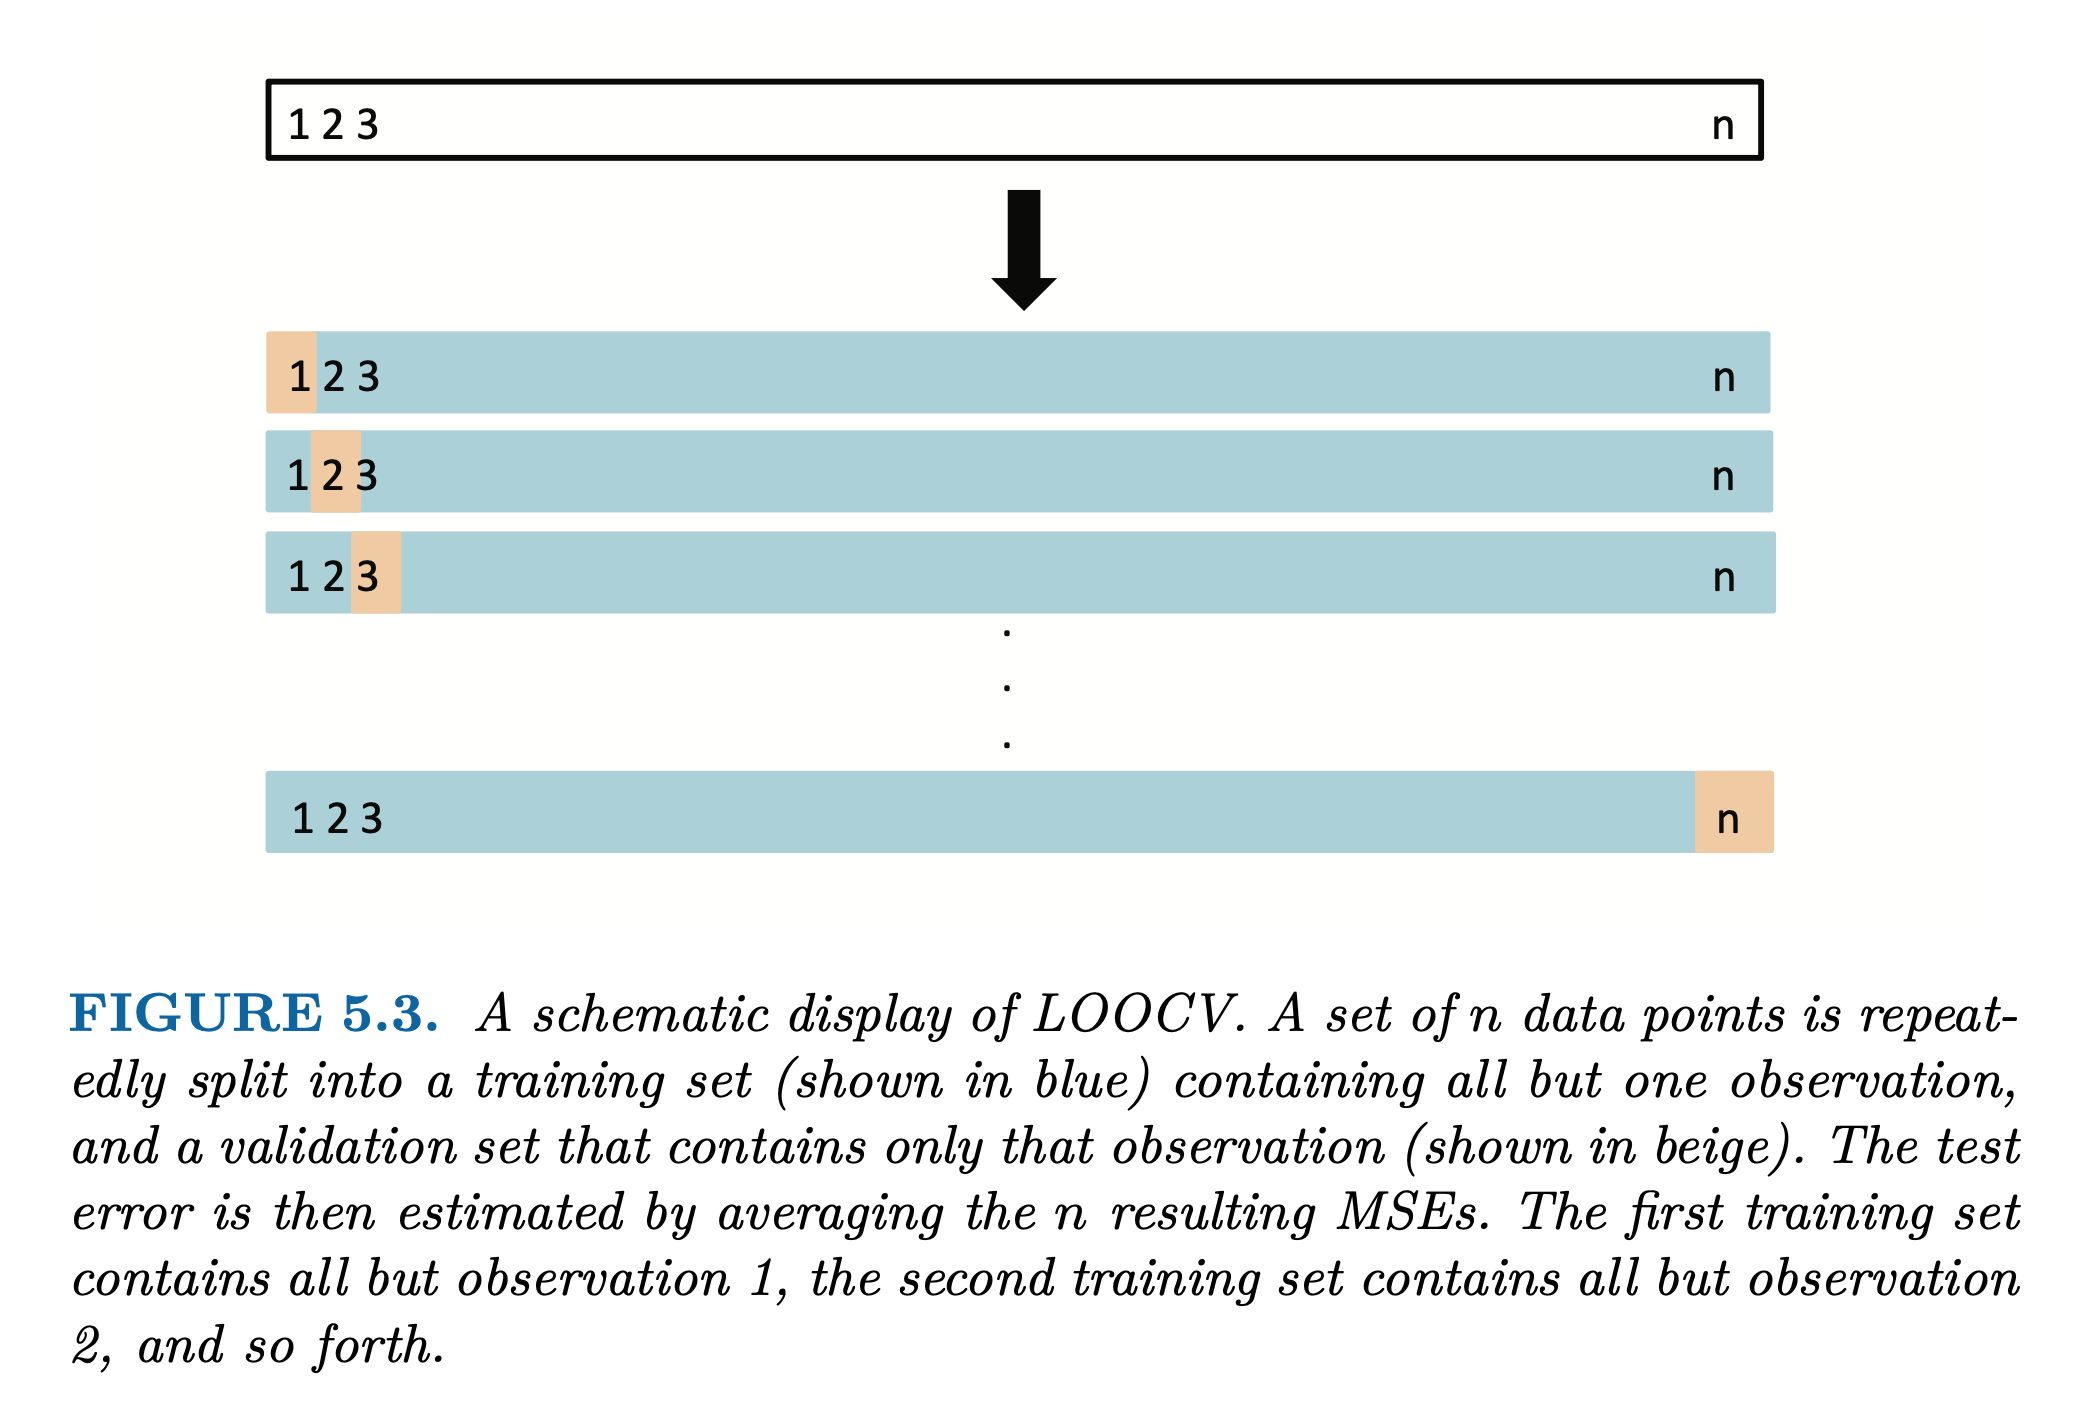
\includegraphics[width = \textwidth]{images/leave_one_out.png}\\
    \hfill \footnotesize Credit: ISLR, page 201
  \end{frame}

  \begin{frame}{$k$-fold cross-validation}
    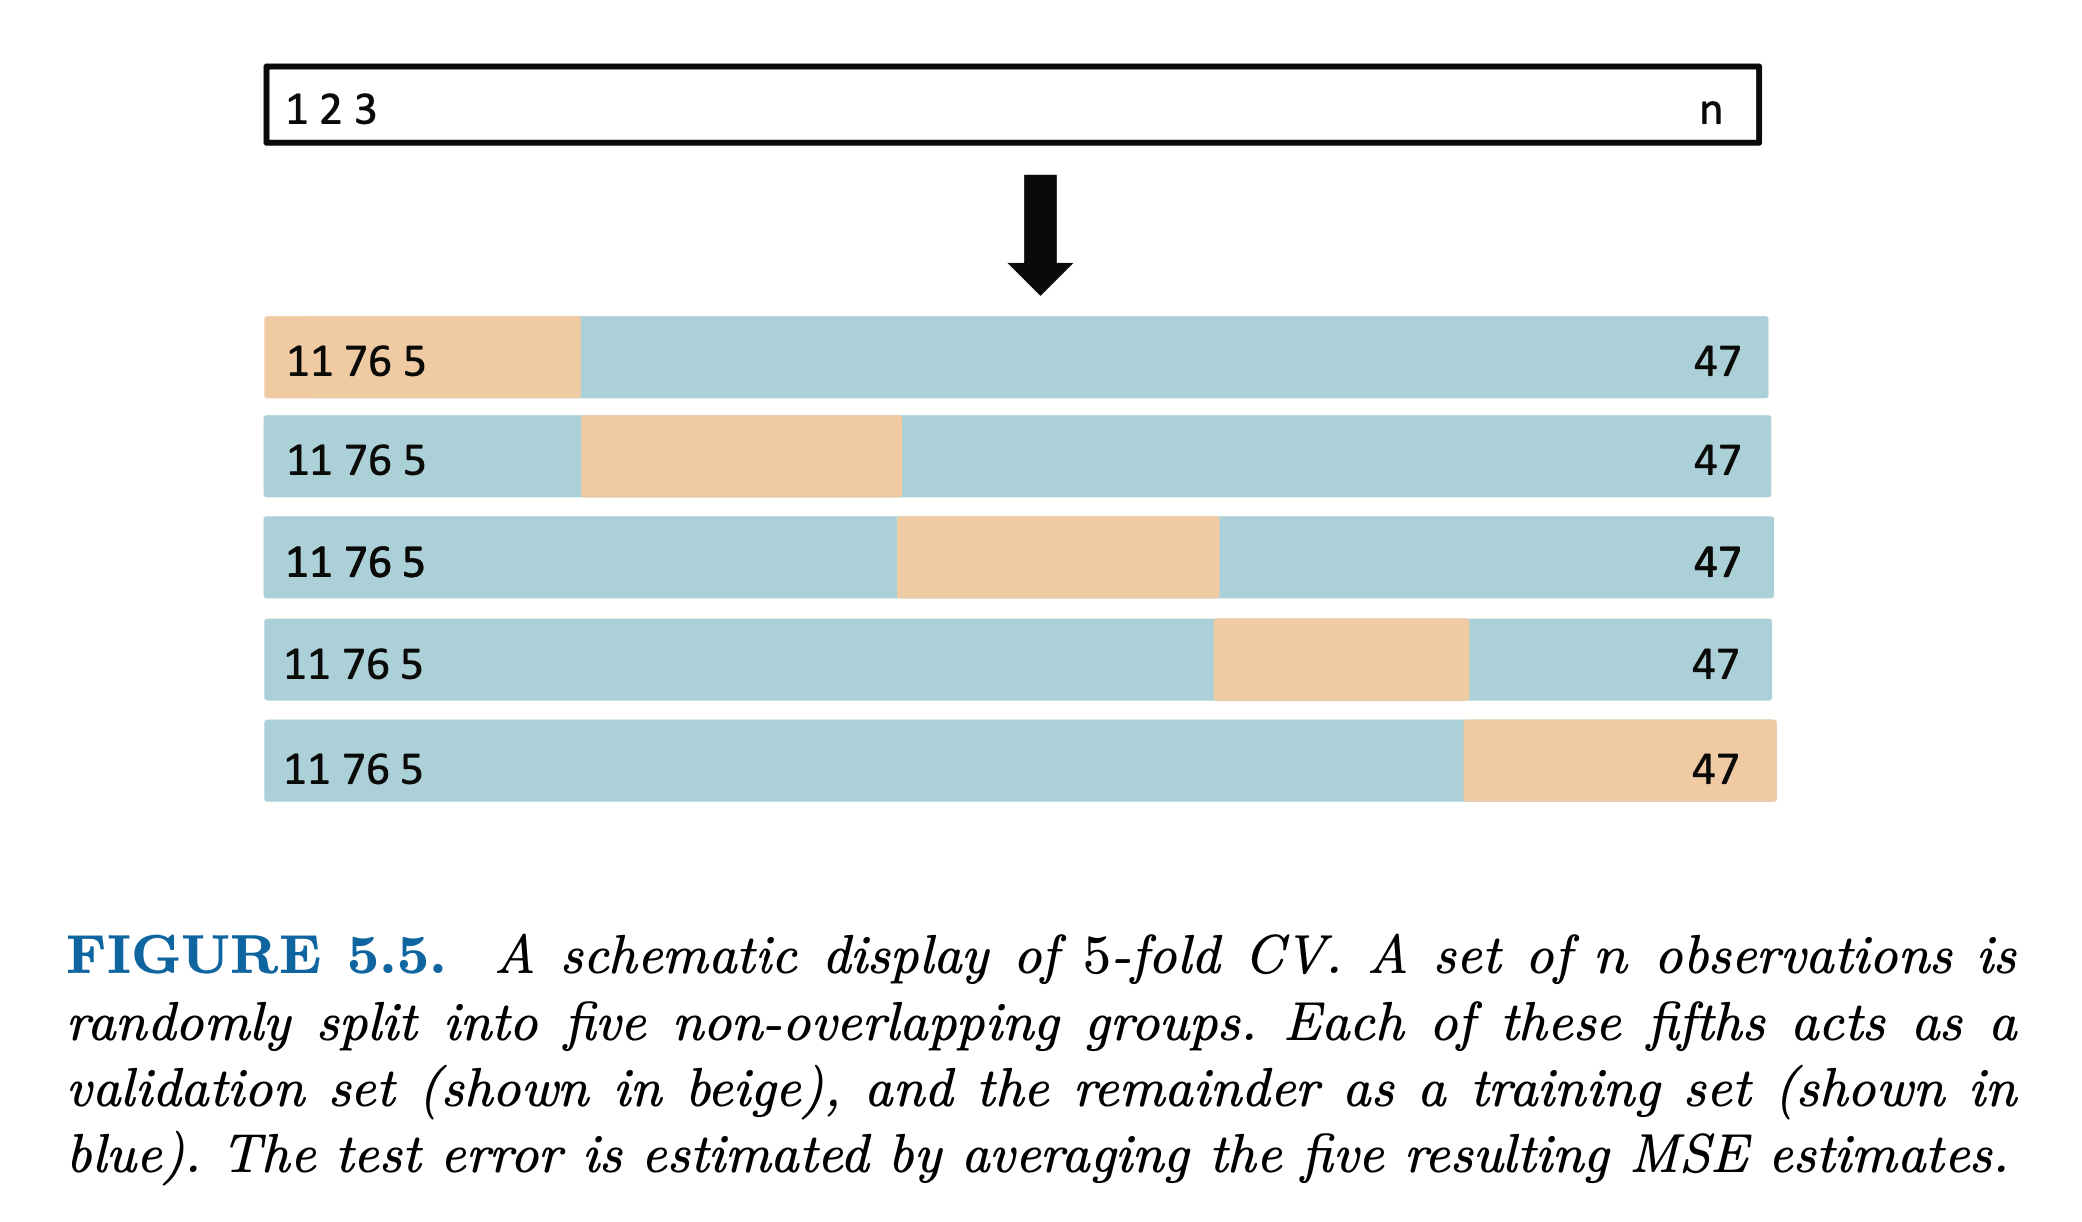
\includegraphics[width = \textwidth]{images/cross_validation.png}\\
    \hfill \footnotesize Credit: ISLR, page 203
  \end{frame}

  \begin{frame}{Example: Cross-validation on the Credit data set}
    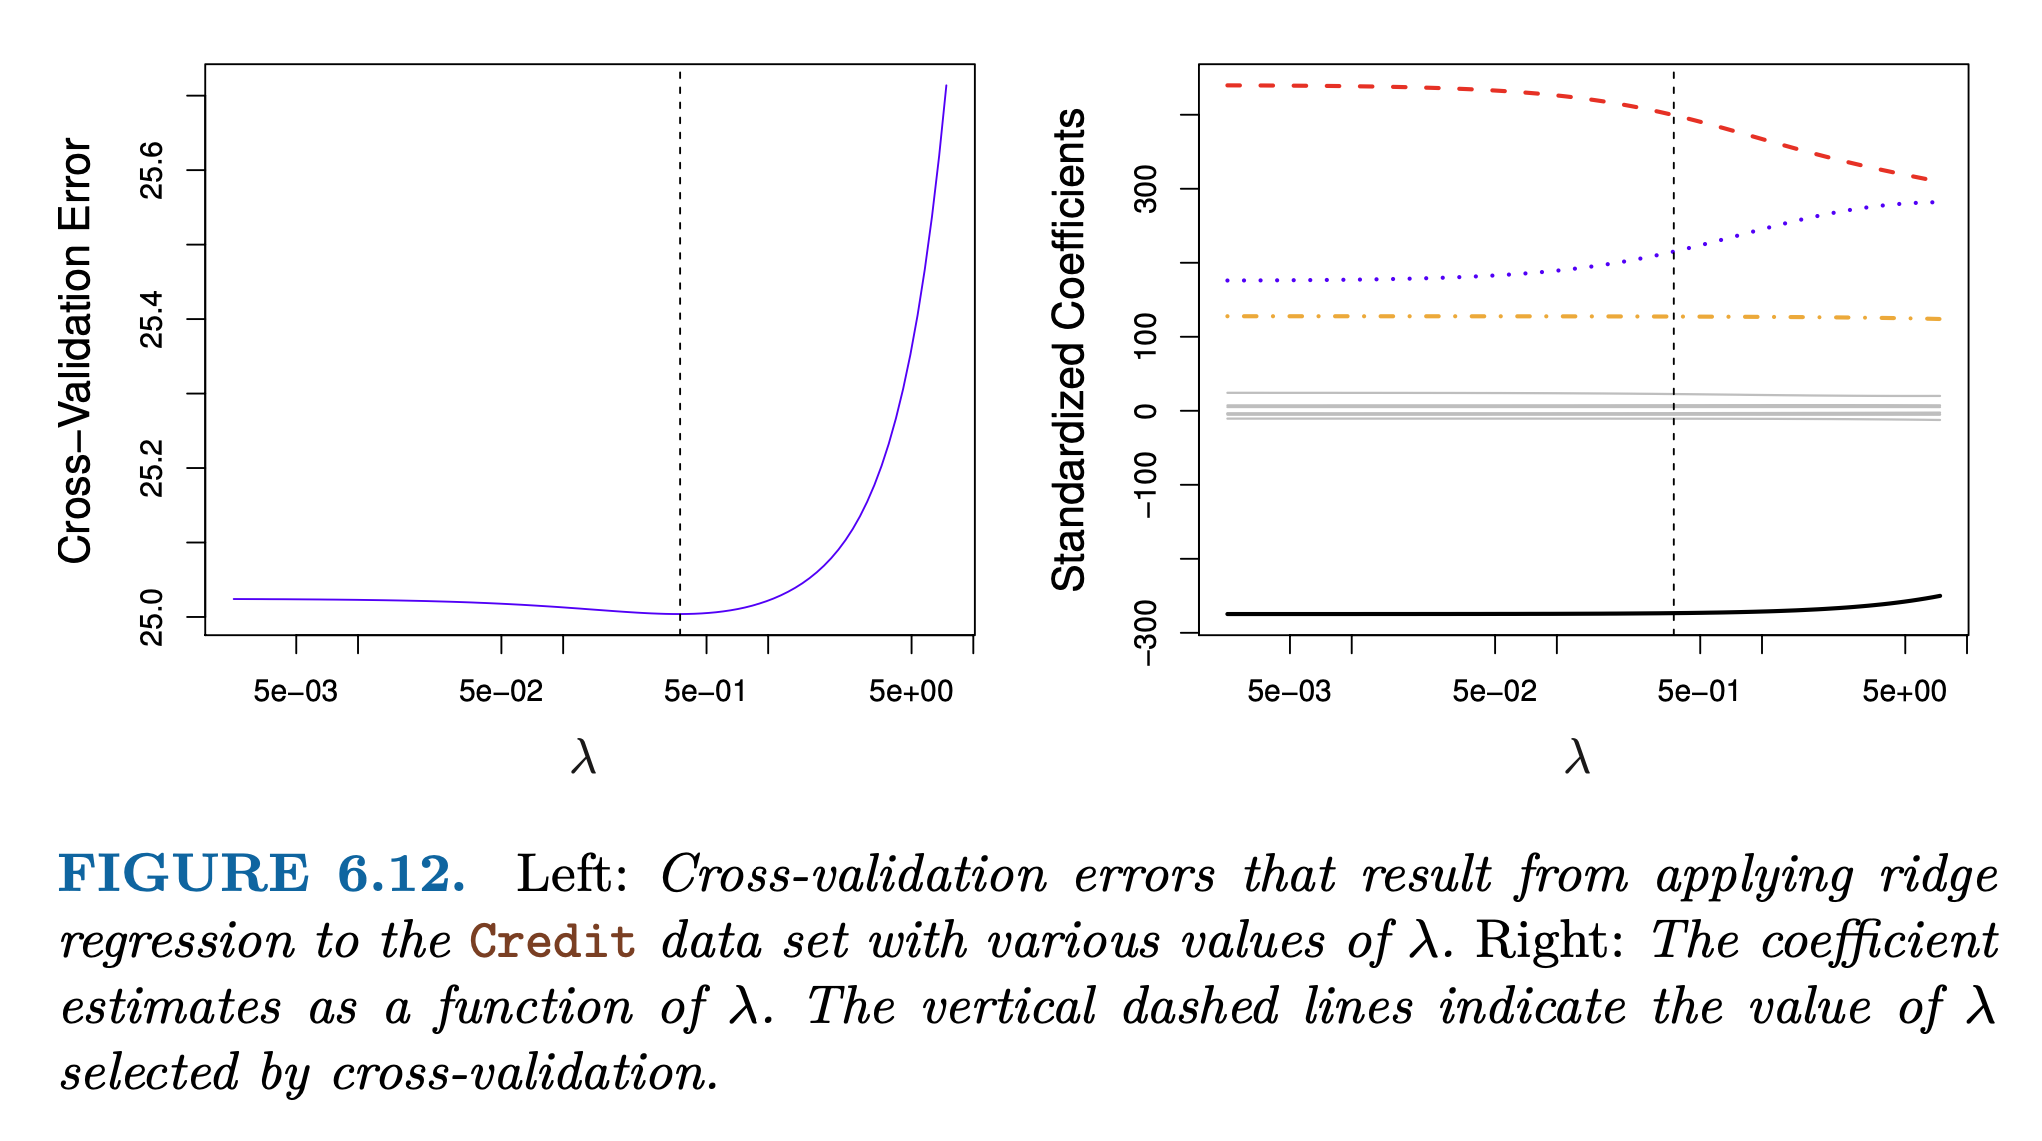
\includegraphics[width = \textwidth]{images/cross_validation_credit.png}
    \vfill
    \hfill \footnotesize Credit: ISLR, page 251
  \end{frame}

  \begin{frame}{Exercise (ISLR, page 220)}
    \begin{itemize}
      \item[(a)] Explain how $k$-fold cross-validation is implemented.
      \item[(b)] What are the advantages and disadvantages of $k$-fold cross-validation relative to:
      \begin{itemize}
        \item[i.] The validation set approach?
        \item[ii.] Leave-one-out cross-validation (LOOCV)?
      \end{itemize}
      \item[(c)] What is the trade-off to consider when choosing $k$ for $k$-fold cross-validation?
    \end{itemize}
  \end{frame}

  \begin{frame}[fragile=singleslide]\frametitle{The glmnet R package}
    \small
    Elastic net regression:
    $$\sum_{i = 1}^n w_i \left(y_i - \beta_0 - \sum_{j = 1}^p \beta_j x_{ij}\right)^2 + (1 - \alpha) \cdot \lambda \sum_{j = 1}^p \beta_j^2 + \alpha \cdot \lambda \sum_{j = 1}^p |\beta_j|$$
    In R:
    \begin{columns}
      \begin{column}{0.5\textwidth}
        \begin{verbatim}
    glmnet::glmnet(
      x,
      y,
      weights = NULL,
      alpha = 1,
      lambda = NULL,
      standardize = TRUE,
      intercept = TRUE,
      ...
    )
      \end{verbatim}
      \end{column}
      \begin{column}{0.5\textwidth}
        \begin{verbatim}
    glmnet::cv.glmnet(
      x,
      y,
      weights = NULL,
      lambda = NULL,
      nfolds = 10,
      foldid = NULL,
      parallel = FALSE,
      ...
    )
      \end{verbatim}
      \end{column}
    \end{columns}
  \end{frame}

  \begin{frame}{Application: Basketball Analytics}
    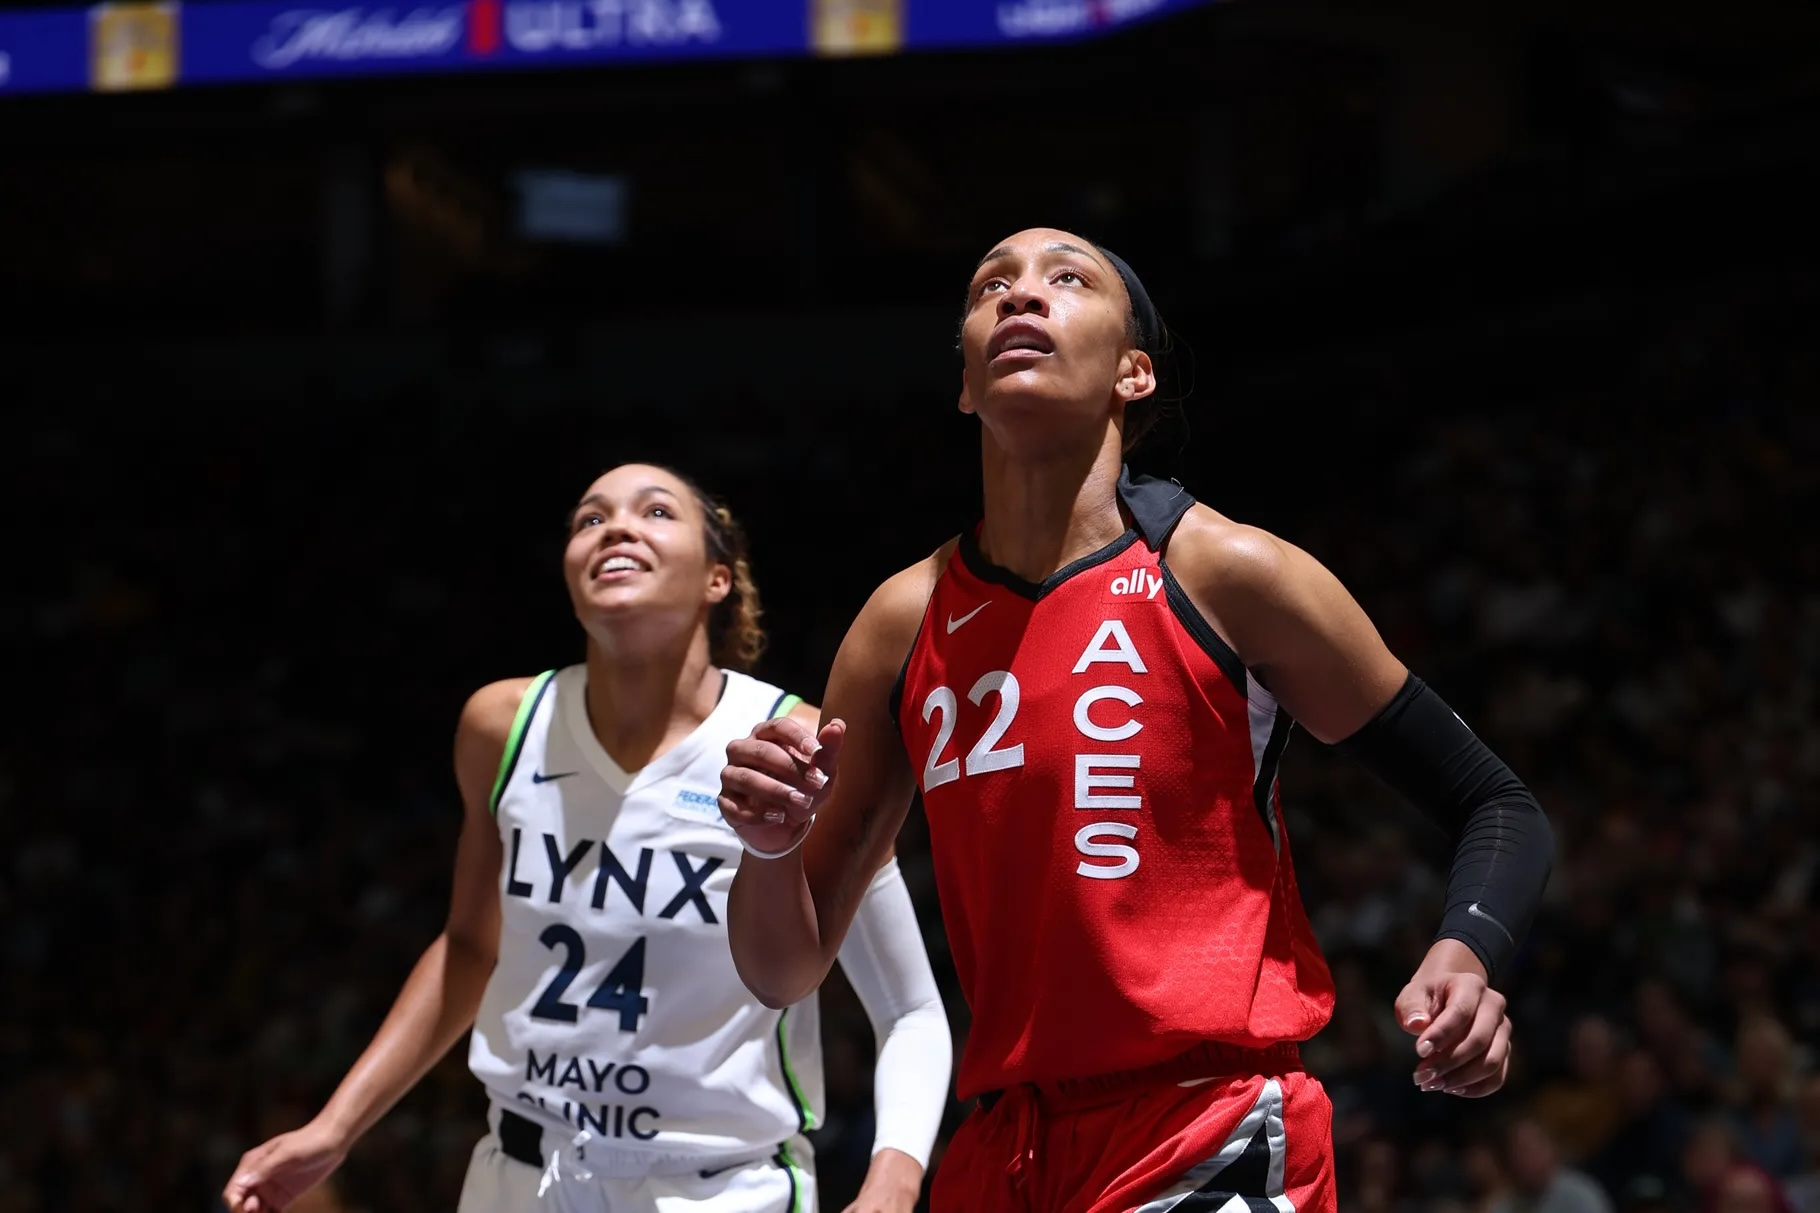
\includegraphics[width = \textwidth]{images/wilson_collier.jpg}
  \end{frame}

  \begin{frame}{Regularized Adjusted Plus-Minus (RAPM)}
    We have {\it stints} (periods of no substitutions) labeled $i = 1, ..., n$
    \begin{itemize}
      \item $w_i$ is the length (in minutes) of stint $i$
      \item $y_i$ is the score differential (home $-$ away) during stint $i$
      \item $H_i$ is the set of home players on the floor during stint $i$
      \item $A_i$ is the set of away players on the floor during stint $i$
    \end{itemize}
    Model:
    $$
      Y_i / w_i = \beta_0 + \sum_{j \in H_i} \beta_j - \sum_{j' \in A_i} \beta_{j'} + \epsilon_i
    $$
    Fitting procedure (ridge regression):
    $$
      \boldsymbol{\hat\beta} = \arg\min_{\boldsymbol{\beta}} \left\{
        \sum_{i=1}^n w_i \left(y_i - \left(\beta_0 + \sum_{j \in H_i}\beta_j - \sum_{j' \in A_i}\beta_{j'}\right)\right)^2 + \lambda \sum_{j = 1}^p \beta_j^2
      \right\}
    $$
  \end{frame}

  \begin{frame}{Framing RAPM as ridge regression}
    We can re-frame this using
    $$
      x_{ij} = \begin{cases}
        +1        & \mbox{ if player $j$ is on the floor for the {\it home} team during stint $i$}\\
        -1        & \mbox{ if player $j$ is on the floor for the {\it away} team during stint $i$}\\
        \hfill 0  & \mbox{ if player $j$ is {\it off} the floor during stint $i$}
      \end{cases}
    $$
    Ridge regression:
    $$
      \boldsymbol{\hat\beta} = \arg\min_{\boldsymbol{\beta}} \left\{
        \sum_{i=1}^n w_i \left(y_i - \left(\beta_0 + \sum_{j = 1}^p x_{ij}\beta_j\right)\right)^2 + \lambda \sum_{j = 1}^p \beta_j^2
      \right\}
    $$
  \end{frame}

  \begin{frame}{Sample X matrix for RAPM}
    $$
      \hspace{-9mm}
      X = \left[
        \begin{array}{*{20}r}
         +1 &+1 &+1 &+1 &+1 & 0 &...&-1 &-1 &-1 &-1 &-1 &...& 0\\
         +1 &+1 &+1 &+1 & 0 &+1 &...&-1 &-1 &-1 &-1 &-1 &...& 0\\
         +1 &+1 &+1 &+1 & 0 &+1 &...&-1 &-1 &-1 & 0 & 0 &...& 0\\
          0 &+1 &+1 &+1 & 0 &+1 &...& 0 &-1 &-1 & 0 & 0 &...& 0\\
          0 &+1 &+1 &+1 &+1 & 0 &...& 0 &-1 &-1 & 0 & 0 &...& 0\\
          0 & 0 & 0 &+1 &+1 & 0 &...& 0 &-1 &-1 &-1 &-1 &...& 0\\
         +1 & 0 & 0 &+1 &+1 & 0 &...&-1 &-1 &-1 &-1 &-1 &...& 0\\
         +1 & 0 & 0 & 0 &+1 &+1 &...&-1 & 0 & 0 &-1 &-1 &...& 0\\
         ...&...&...&...&...&...&...&...&...&...&...&...&...&...\\
          0 & 0 & 0 &+1 &+1 & 0 &...& 0 & 0 & 0 & 0 & 0 &...& 0\\
         +1 & 0 & 0 &+1 &+1 & 0 &...& 0 & 0 & 0 & 0 & 0 &...& 0\\
         +1 & 0 & 0 &+1 & 0 &+1 &...& 0 & 0 & 0 & 0 & 0 &...& 0\\
         ...&...&...&...&...&...&...&...&...&...&...&...&...&...\\
          0 & 0 & 0 & 0 & 0 & 0 &...& 0 & 0 & 0 & 0 & 0 &...& 0\\
        \end{array}
      \right]
    $$
    \begin{itemize}
      \item This matrix is very {\it sparse} (most of the entries are zero)
    \end{itemize}
  \end{frame}

  \begin{frame}[fragile=singleslide]\frametitle{3 glmnet lessons I learned the hard way}
    \begin{columns}
      \begin{column}{0.35\textwidth}
        \begin{verbatim}
glmnet::glmnet(
  x,
  y,
  weights = NULL,
  alpha = 1,
  lambda = NULL,
  standardize = TRUE,
  intercept = TRUE,
  ...
)
        \end{verbatim}
      \end{column}
      \begin{column}{0.65\textwidth}
        \begin{enumerate}
          \item For ridge regression, use {\tt alpha = 0}.
          \item Check whether the default {\tt lambda} range includes the optimal value for you
            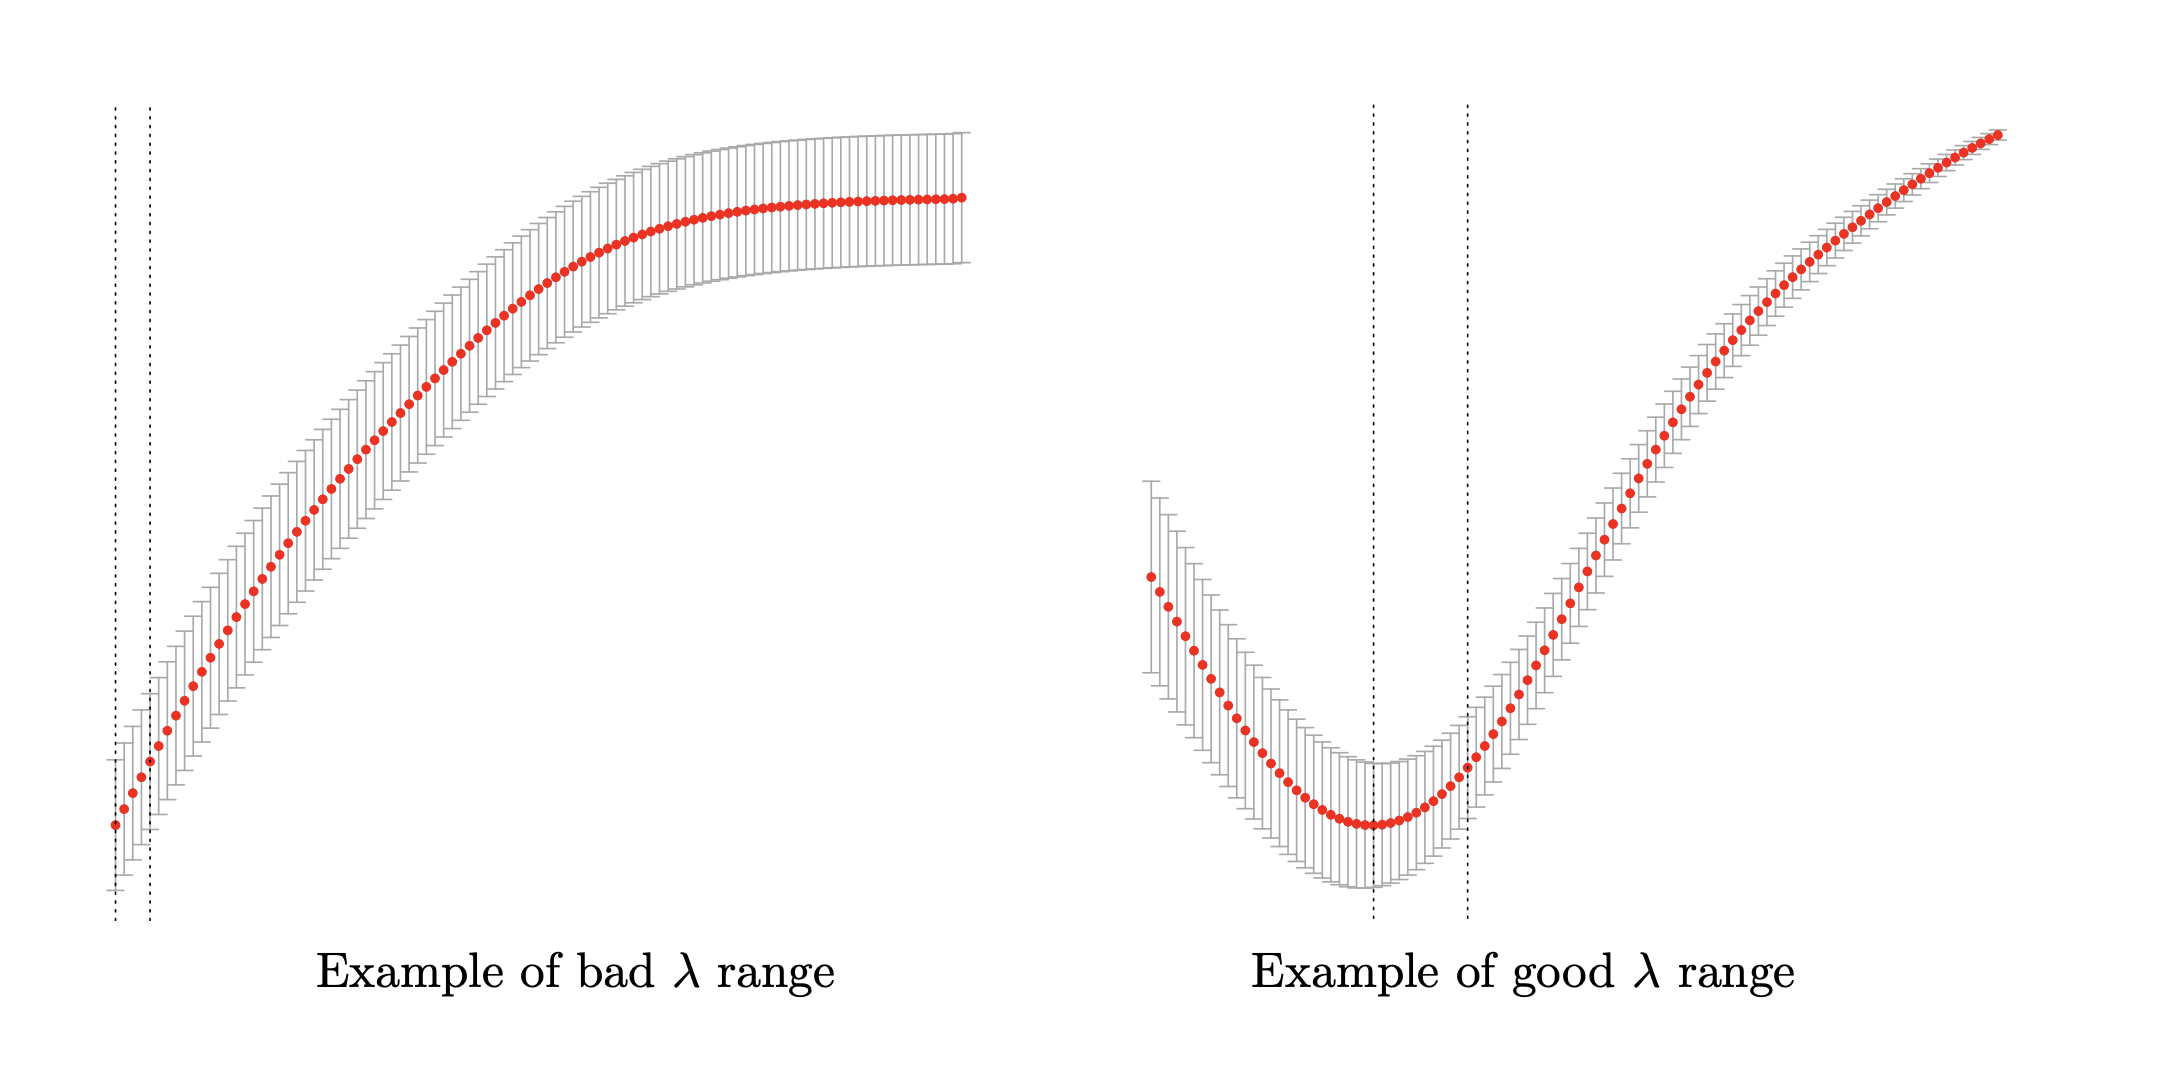
\includegraphics[width = \textwidth]{images/lambda_range.png}
          \item For RAPM, {\tt standardize = FALSE}.
        \end{enumerate}
      \end{column}
    \end{columns}
  \end{frame}

  \begin{frame}{Google Colab}
    Ground rules:
    \begin{enumerate}
      \item After opening the Google Colab notebook, select ``File'' $\rightarrow$ ``Save a Copy in Drive''. This will open a new tab with a version you can edit and save. If you keep the original open in a separate tab, you can refresh it to see updates I post.
      \item Next, select ``Runtime'' $\rightarrow$ ``Change runtime type'', and change the runtime type from Python 3 to R.
      \item Now you can get started! Raise your hand or ask a neighbor when you feel stuck or lost. The first two code blocks take several minutes to run, so start thinking ahead while they run.
    \end{enumerate}
  \end{frame}

\end{document}
